To further discuss the details of the algorithm, we used it on a smaller version of the problem. Let there be a 1km by 1km land area for the wind farm and for the whole year, the wind blows with constant wind speed of $12\;m/s$ on all wind directions that are multiples of $10^o$ (i.e. $0^o,$, $10^o$, $20^0$ $,...,$ + $340^o$, $350^o$) with equal fraction of occurrences of $\frac{1}{36}$ for a total of $1$. Using our model for the wind farm, this 1000 meter by 1000 meter wind farm would have a matrix model (binary and real) with 5 rows and 5 columns, resulting to 25 possible turbine locations.

    
 \section{Exhaustive Search}
    To determine the effectiveness of the algorithm, it is possible to find the optimal solution for the smaller scale of the problem by exhaustively searching all the possible solution from 1 wind turbine up to 25 wind turbines. Then compare the optimal solution given by the proposed algorithm with the optimal solution given by the exhaustive search to test if the proposed algorithm indeed gives the right optimal solution for the problem.
    
    Note that the number of the search elements $S$ for the exhaustive search is the number of all possible combinations of $N$ wind turbines on the $25$ possible wind turbine locations on the $1km\;by\;1km$ wind farm, computed as
    \begin{align*}
        S
        &= \sum_{N-1}^{25}\binom{25}{N} = \sum_{N-1}^{25}\frac{25!}{N(25-N)!} \\
        &= \binom{25}{1} + \binom{25}{2} + \binom{25}{3} + \binom{25}{4} +...+ \binom{25}{25} \\
        &= \frac{25!}{1(25-1)!} + \frac{25!}{2(25-2)!} + \frac{25!}{3(25-3)!} + \frac{25!}{4(25-4)!} +..+ \frac{25!}{25(25-25)!} \\
        &= 25+300+2300+12650+...+1 \\
        &= 33\;554\;431
    \end{align*}
    
    Considering the size of the search space for such smaller scale of the problem, it would be almost impossible to perform an exhaustive search for bigger scale of the problem.
    
    For the $N=1$ number of wind turbines, the total power output of the whole farm should be the same wherever that single wind turbine is placed because it is assumed that the wind speed is the same for all locations on the wind farm. For a constant wind speed of $12m/s$, the wind farm with a single wind turbine has a total power of
        \begin{align*}
            P_{tot}=P
            &= 0.3u^3 \\
            &= 0.3(12\;m/s)^3\\
            &= 518.4 \;kW
        \end{align*}
        
    For $N=2$ wind turbines, it is important to determine first which wind turbine is the upstream and which wind turbine is the downstream. Let there be two wind turbines $T_1$ and $T_2$ located at $(i_1,j_1)$ and $(i_2,j_2)$ respectively. Given a wind direction of $\theta$, $T_1$ is the upstream wind turbine if the coordinates of both wind turbines satisfy the conditions in Table \ref{coverage1}, and $T_2$ is the upstream wind turbine if the coordinates of both wind turbines satisfy the conditions in Table \ref{coverage2}.
    
    \begin{table}[h]
        \centering
        \begin{tabular}{|c|c|} \hline
            Wind direction $\theta$ & $T_1$ is upstream if \\ \hline
            $\theta = 0^o$ & $i_1<i_2$ \\ \hline
            $0^o<\theta<90^o$ & $i_1 \leq i_2 \;AND\; j_1 \leq j_2$ \\ \hline
            $\theta = 90^o$ & $j_1<j_2$ \\ \hline
            $90^o<\theta<180^o$ & $i_1 \geq i_2 \;AND\; j_1 \leq j_2$ \\ \hline
            $\theta = 180^o$ & $i_1>i_2$ \\ \hline
            $180^o<\theta<270^o$ & $i_1 \geq i_2 \;AND\; j_1 \geq j_2$ \\ \hline
            $\theta = 270^o$ & $j_1>j_2$ \\ \hline
            $270^o<\theta<360^o$ & $i_1 \leq i_2 \;AND\; j_1 \geq j_2$ \\ \hline
        \end{tabular}
        \caption{Conditions for turbine $T_1$ to be upstream given two wind turbines $T_1$ and $T_2$ located at $(i_1,j_1)$ and $(i_2,j_2)$ respectively.}
        \label{coverage1}
    \end{table}
    
    \begin{table}[h]
        \centering
        \begin{tabular}{|c|c|} \hline
            Wind direction $\theta$ & $T_2$ is upstream if \\ \hline
            $\theta = 0^o$ & $i_1>i_2$ \\ \hline
            $0^o<\theta<90^o$ & $i_1 \geq i_2 \;AND\; j_1 \geq j_2$ \\ \hline
            $\theta = 90^o$ & $j_1>j_2$ \\ \hline
            $90^o<\theta<180^o$ & $i_1 \leq i_2 \;AND\; j_1 \geq j_2$ \\ \hline
            $\theta = 180^o$ & $i_1<i_2$ \\ \hline
            $180^o<\theta<270^o$ & $i_1 \leq i_2 \;AND\; j_1 \leq j_2$ \\ \hline
            $\theta = 270^o$ & $j_1<j_2$ \\ \hline
            $270^o<\theta<360^o$ & $i_1 \geq i_2 \;AND\; j_1 \leq j_2$ \\ \hline
        \end{tabular}
        \caption{Conditions for turbine $T_2$ to be upstream given two wind turbines $T_1$ and $T_2$ located at $(i_1,j_1)$ and $(i_2,j_2)$ respectively.}
        \label{coverage2}
    \end{table}
    
    If the both of them are not upstream wind turbines, then both of them experience the original wind speed of $u_\infty$ and have a power output of
    \begin{equation}
        P_1=P_2=0.3u_\infty^3
    \end{equation}
    where $P_1$ is the power output of wind turbines $T_1$ and $P_2$ is the power output of wind turbine $T_2$. The same power output will be experienced by a wind turbines as long as it is an upstream one. However, if one of them is not an upstream wind turbines, this wind turbine has a chance of being affected by the wake of the upstream wind turbine.
    
    Considering the locations of wind turbines $T_1$ and $P_2$ where one of them is upstream, equation \ref{xSmall} becomes
    \begin{equation} \label{xSmall}
        x =
        \begin{cases} 
            \left(200m\cdot\sqrt{\left| \Delta i \right|^2+\left| \Delta j \right|^2}\right)cos\left(90^o-tan^{-1}\left| \frac{\left| \Delta j \right|}{\left| \Delta i \right|} \right| \right) & \theta \neq 90^o \;AND\; \theta \neq 270^o \\
            \left(200m\cdot\sqrt{\left| \Delta i \right|^2+\left| \Delta j \right|^2}\right)cos\left( \left( \theta \;mod\; 90^o \right)-tan^{-1}\left| \frac{\left| \Delta j \right|}{\left| \Delta i \right|} \right| \right) & elsewhere
        \end{cases}
    \end{equation}
    where $\Delta i=|i_1-i_2|$ and $\Delta j=|j_1-j_2|$.
    
    Let the functions $P_1(i_1,j_1,i_2,j_2,\theta,u_\infty)$ and $P_2(i_1,j_1,i_2,j_2,\theta,u_\infty)$ give the power output of wind turbines $T_1$ and $T_2$ respectively. If $y<=r$ then the modified Jensen's Model applies on the downstream wind turbine. Hence $P_1$ and $P_2$ are given by
    \begin{equation}
        P_1(i_1,j_1,i_2,j_2,\theta,u_\infty) =
        \begin{cases} 
            0.3u_\infty^3 & C1 \;is\;true \\
            0.3u_\infty^3 & y > r \\
            0.3\left[ u_\infty\left(1 - 2a\left(\frac{r_{1}}{r_{1}+\beta x}\right)^2\right) \right]^3 & otherwise
        \end{cases}
    \end{equation}
    \begin{equation}
        P_2(i_1,j_1,i_2,j_2,\theta,u_\infty) =
        \begin{cases} 
            0.3u_\infty^3 & C2 \;is\;true \\
            0.3u_\infty^3 & y > r \\
            0.3\left[ u_\infty\left(1 - 2a\left(\frac{r_{1}}{r_{1}+\beta x}\right)^2\right) \right]^3 & otherwise
        \end{cases}
    \end{equation}
    where $C1$ is true if $T_1$ is upstream OR both $T_1$ and $T_2$ are not upstream wind turbines, $C2$ is true if $T_2$ is upstream OR both $T_1$ and $T_2$ are not upstream wind turbines, and x is computed in equation \ref{xSmall}.
    
    %SHOW THE SPECS AND VARIABLE VALUES
    Moreover, the specification and wind farm assumptions for the wind turbine used for the study of Abdelsalam et al. \cite{this} are shown in Table \ref{turbineSpecs}. Using the thrust coefficient of the considered wind turbine, it follows that the Axial Induction Factor $a$ is
    \begin{align*}
        a
        &=0.5-0.5\sqrt{1-C_T} \\
        &=0.5-0.5\sqrt{1-0.88} \\
        a &= 0.3267949
    \end{align*}
    Also, the entrainment constant $\beta$ and $r_1$ for the the modified Jensen's wake model are as follows.
    \begin{align*}
        \beta
        &=\frac{0.5}{ln(z/z_o)} \\
        &=\frac{0.5}{ln(60m/0.3m)} \\
        &=0.9437
    \end{align*}
    \begin{align*}
        r_1
        &=r_o\sqrt{\frac{1-a}{1-2a}} \\
        &=(20m)\sqrt{\frac{1-0.3267949}{1-2(0.3267949)}} \\
        &=27.881\;meters
    \end{align*}
        
    \begin{table}[H]
        \centering
        \begin{tabular}{|l|c|} \hline
            Hub Height $z$ & 60 meters \\ \hline
            Ground Roughness $z_o$ & 0.3 meters \\ \hline
            Rotor Radius $r_o$ & 20 meters \\ \hline
            Thrust Coefficient $C_T $ & 0.88 \\ \hline
        \end{tabular}
        \caption{Specifications of the considered wind turbine and Assumptions for the wind farm.}
        \label{turbineSpecs}
    \end{table}
    
    \begin{figure}[H]
        \centering
        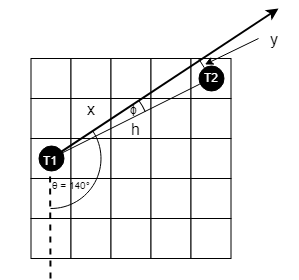
\includegraphics[width=0.5\linewidth]{Figures/sampleSmall1.png}
        \caption{An example of wind farm configuration with two wind turbines.}
        \label{sampleSmall1}
    \end{figure}
    
    For example, consider the same wind farm with two wind turbines $T_1$ and $T_2$ located at $(2,0)$ and $(0,4)$, wind direction at $\theta=140^o$ and wind speed of $12m/s$. The schematics of the said wind farm is shown in Figure \ref{sampleSmall1}. The hypotenuse of the triangle showed on the figure labelled as $h$ has a length of
    \begin{align*}
    	h
    	&= (200m)\cdot \sqrt{(2-0)^2+(0-4)^2} \\
    	&= (200m)\cdot \sqrt{20} \\
    	&= 894.427\;meters
    \end{align*}
    Also, the angle labelled as $\phi$ from the figure has a magnitude of
    \begin{align*}
    	\phi
    	&= tan^{-1} \left| \frac{0-4}{2-0} \right| \\
    	&= tan^{-1} 2 \\
    	&= 63.435^o
    \end{align*}
    It follows that the distance between the two turbines with respect to the direction of wind has a magnitude of
    \begin{align*}
    	x
    	&= (894.427m)\cdot cos\left| (140^o\;mod\;90^o)-63.435^o \right| \\
    	&= (894.427m)\cdot cos\left| 50^o-63.435^o \right| \\
    	&= 869.950\;meters
    \end{align*}
    And the the line segment labelled as $y$ from the figure has a magnitude of
    \begin{align*}
    	y
    	&= (894.427m)\cdot sin\left| (140^o\;mod\;90^o)-63.435^o \right| \\
    	&= (894.427m)\cdot sin\left| 50^o-63.435^o \right| \\
    	&= 207.813\;meters
    \end{align*}
    which is less than the resulting radius of the wake $870.242\;meters$ away from the upstream wind turbine as computed below.
    \begin{align*}
    	r
    	&= (0.3267949)(870.242m) + 20m \\
    	&= 304.295\;meters
    \end{align*}
    
    Using the modified Jensen's wake model, the wind speed experienced by the downstream wind turbine $T_2$ is
    \begin{align*}
    	u_2
    	&= (12m/s)\left[ 1-2(0.3267949)\left( \frac{27.881m}{27.881m+(0.09437)(869.950m)} \right)^2 \right] \\
    	&= 11.496m/s
    \end{align*}
    and a power output of
    \begin{align*}
    	P_2(2,0,0,4,140^o,12m/s)
    	&= 0.3u_2^3 \\
    	&= 0.3(11.469m/s)^3 \\ 
    	&= 455.787kW
    \end{align*}
    while the upstream wind turbine $T_1$ has a power output of
    \begin{align*}
    	P_1(2,0,0,4,140^o,12m/s)
    	&= 0.3u_2^3 \\
    	&= 0.3(12m/s)^3 \\ 
    	&= 518.4kW
    \end{align*}
    
    \begin{figure}[H]
        \centering
        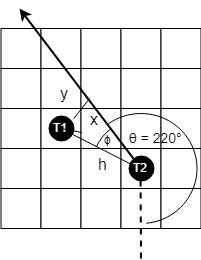
\includegraphics[width=0.4\linewidth]{Figures/sampleSmall2.png}
        \caption{An example of wind farm configuration with two wind turbines.}
        \label{sampleSmall2}
    \end{figure}
    
    Another configuration of the 1km by 1km wind farm with two wind turbines is shown in Figure \ref{sampleSmall2} where the wind direction is at $\theta=220^o$, wind turbines $T_1$ and $T_2$ located at $(1,2)$ and $(3,3)$ respectively, and a wind speed of $12m/s$. Using the generalized formula for y, the line segment labelled as $y$ from the figure has a length of
    \begin{align*}
    	y
    	&= \left((200m)\cdot \sqrt{(1-3)^2+(2-3)^2}\right)\cdot sin\left| (220^o\;mod\;90^o)-tan^{-1} \left| \frac{2-3}{1-3} \right| \right| \\
    	&= 103.907\;meters
    \end{align*}
    which is less than the resulting radius of the wake at the distance of the downstream wind turbine $T_1$. That is,
    \begin{align*}
    	r
    	&= (0.3267949)\left[ \left((200m)\cdot \sqrt{(1-3)^2+(3-3)^2}\right)\cdot sin\left| (220^o\;mod\;90^o)-tan^{-1} \left| \frac{0-4}{2-0} \right| \right| \right] + 20m \\
    	&= 162.148\;meters
    \end{align*}
    This means that wind turbine $T_1$ is affected by the wake of the upstream wind turbine $T_2$ at a wind direction of $\theta=220^o$. Using the generalized formula for the power output of the two turbines, the power output of the wind turbines are as follows.
    \begin{align*}
        x
        &=\left((200m)\cdot \sqrt{(1-3)^2+(2-3)^2}\right)\cdot cos\left| (220^o\;mod\;90^o)-tan^{-1} \left| \frac{2-3}{1-3} \right| \right| \\
        &=434.976\;meters
    \end{align*}
    \begin{align*}
    	P_1(1,3,2,3,220^o,12m/s)
    	&= 0.3\left[ u_\infty\left(1 - 2(0.3267949)\left(\frac{(27.881m)}{(27.881m)+(0.9437) (434.976m)}\right)^2\right) \right]^3 \\
    	&= 369.276\;kiloWatts
    \end{align*}
    \begin{align*}
    	P_2(1,3,2,3,220^o,12m/s)
    	&= 0.3u_2^3 \\
    	&= 0.3(12m/s)^3 \\ 
    	&= 518.4\;kiloWatts
    \end{align*}
    
    \begin{figure}[H]
        \centering
        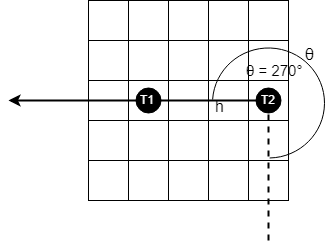
\includegraphics[width=0.5\linewidth]{Figures/sampleSmall3.png}
        \caption{An example of wind farm configuration with two wind turbines.}
        \label{sampleSmall3}
    \end{figure}
    
    Notice that the formula for $\phi$ is expressed as a quotient which would be invalid if the two turbines are positioned on the same row. However, it would still be usable for that case. Consider the wind farm shown in Figure \ref{sampleSmall3}, where the wind turbines $T_1$ and $T_2$ are located at $(2,1)$ and $(2,4)$ respectively, and a wind speed of $12m/s$ blowing at a direction of $\theta=270^o$. By looking at the figure, the distance between the two figure with respect to the direction of the wind is trivial, that is
    \begin{align*}
    	x
    	&= 200\cdot |j_1-j_2| \\
    	&= 200\cdot |1-4| \\ 
    	&= 600\;meters
    \end{align*}
    and the 'y' segment is not visible because it has a length of 0, which makes it obvious that the wind turbine $T_1$ is affected by the wake of the upstream wind turbine $T_2$. Therefore, the wind speed experienced by the downstream wind turbine is
    \begin{align*}
    	u_1
    	&= (12m/s)\left(1 - 2(0.3267949)\left(\frac{(27.881m)}{(27.881m)+(0.9437)(600m)}\right)^2\right) \\
    	&= 11.146\;m/s
    \end{align*}
    and a power output of
    \begin{align*}
    	P_1(2,2,1,4,270^o,12m/s)
    	&= 0.3u_1^3 \\
    	&= 0.3(11.146m/s)^3 \\ 
    	&= 415.411kW
    \end{align*}
    
    However, the generalized formula should always work regardless of the locations of the wind turbines. The problem with the division by zero for computing the angle $\phi$ can be fixed by determining what value the inverse tangent would approach if the denominator of the expression approaches to zero.
    \begin{align*}
    	\phi
    	&= tan^{-1} \left| \frac{1-4}{2-2} \right| \\
    	&= \lim_{\delta -> 0} \left( tan^{-1} \frac{3}{\delta} \right) \\
    	&= 90^o
    \end{align*}
    Using the value of $\phi$ above and the generalized formula for $x$, the distance $x$ would be
    \begin{align*}
    	x
    	&= \left( (200m)\sqrt{{(2-2)^2+(1-4)^2}} \right)\cdot cos\left| 90^o-90^o \right| \\
    	&= (600m)\cdot cos\left( 0^o \right) \\
    	&= 600\;meters
    \end{align*}
    Thus, it would give the same power output.
    
    \subsection{Best Configuration of Two Wind Turbines}
    
    Considering all possible locations of two wind turbines, the exhaustive search found a total of 300 different configurations. Two of which are found to have the highest total power output where the two wind turbines are located at opposite corners of the wind farms as shown in Figure \ref{small2}.
    
    \begin{figure}[h]
        \centering
        \subfloat{{
\includegraphics[width=6cm]{Figures/Chromosomes/2a.png} }}
        \qquad
        \subfloat{{
\includegraphics[width=6cm]{Figures/Chromosomes/2b.png} }}
        \caption{Best configurations of the small scale problem with 2 wind turbines using exhaustive search method}
        \label{small2}
    \end{figure}
    
    Considering the wind farm on left of Figure \ref{small2}, let $T_1$ be the wind turbine located at $(0,0)$ and $T_2$ be the wind turbine located at $(4,4)$, Figure \ref{bestSmall} shows the schematics of the best configuration for every wind direction.
    
    \begin{figure}[H]
        \centering
        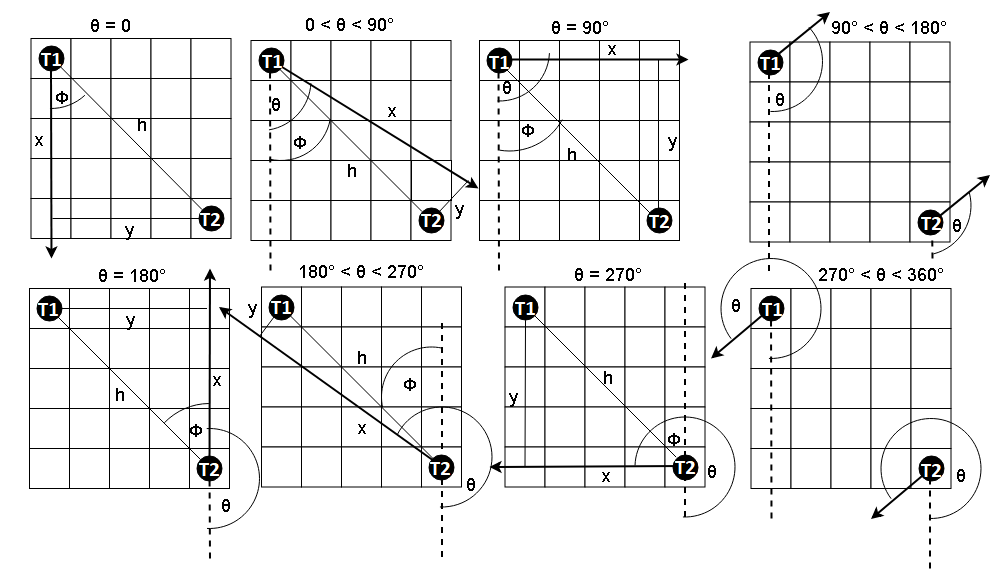
\includegraphics[width=\linewidth]{Figures/bestSmall.png}
        \caption{Schematics of a best configuration of a 1km by 1km wind farm with two wind turbines located at $(0,0)$ and $(4,4)$ for different wind directions.}
        \label{bestSmall}
    \end{figure}

    Note that the distance between the two wind turbines can be solved using their position on the matrix. using the example above, by distance formula where $(i_{1},j_{1})$ is the position of the first wind turbine and $(i_{2},j_{2})$ is the position of the second wind turbine and also considering that each cell in the matrix have $200mx200m$ dimension,
        \begin{align*}
            h &= 200m\cdot \sqrt{(i_{2}+i_{1})^{2}+(j_{2}+j_{1})^{2}}\\
             &= 200m\cdot \sqrt{(4+0)^{2}+(4+0)^{2}} \\
             &= 200m\cdot \sqrt{4^{2}+4^{2}} \\
             &= 200m(5.6568) \\
             &= 1131.3708\;meters
        \end{align*}
    Where h is the distance between the two wind turbines. Now that the actual distance between the wind turbine is determined, the length of the two legs of the right triangle formed by the wind direction and the $h$ as the hypotenuse is solved. Using the given figure, the $\theta=0^{o}$ and $\phi=45^{o}$ where the $\theta$ is the angle of the wind direction and $\phi$ is the angle from the reference point of the first wind turbine to $h$,the $x$ is solved by
        \begin{align*}
            x &= h(cos|(\theta\;mod\;90^{o})-\phi|) \\
              &= 1137.37m(cos|0^{o}-45^{o}|) \\
              &= (1137.37m)(0.7071) \\
            x &= 800m
        \end{align*}
    and the $y$ is
        \begin{align*}
            y &= h(sin|(\theta\;mod\;90^{o})-\phi|) \\
              &= h(1137.37m)(0.7071) \\
            y  &= 800m
        \end{align*}
    Since the $x=800m$, the resulting radius of the wake of the first wind turbine, $T_{1}$ is
        \begin{align*}
            r(x)   &= ax + r_{o} \\
            r(800) &= (0.3267545)(800m) + 20m \\
            r(800) &= 281.436m
        \end{align*}
    where $a$ is the axial induction factor and $r_{0}$ is the rotor radius of the wind turbine. Since $y>r$, the wake of the first wind turbine will not affect the second wind turbine thus there is no wake interaction between the two turbines. Therefore the total power of both turbines using $u_{\infty}=12m/s$ as the wind speed is
        \begin{align*}
            P_{tot} &= P_{1} + P_{2} = 0.3u_{\infty}^{3} + 0.3u_{\infty}^{3} \\
            P_{tot} &= 0.3(12m/s)^{3} + 0.3(12m/s)^{3} \\
            P_{tot} &= 518.4kW + 518.4kW\\
            P_{tot} &= 1036.8kW
        \end{align*}
        
    Now we consider if the wind directions is $0<\theta<90^{o}$. The position of the $x$ and $y$ will change and so is their length. Below shows the length of $x$ and $y$
    different wind direction at $0<\theta<90$   
        \begin{align*}
            x_{\theta=10^{o}} = x_{\theta=80^{o}} &= (1131.37m)cos|10^{o}-45^{o}| &= 926.765m \\ 
            x_{\theta=20^{o}} = x_{\theta=70^{o}} &= (1131.37m)cos|20^{o}-45^{o}| &= 1025.370m \\ 
            x_{\theta=30^{o}} = x_{\theta=60^{o}} &= (1131.37m)cos|30^{o}-45^{o}| &= 1092.820m \\ 
            x_{\theta=40^{o}} = x_{\theta=50^{o}} &= (1131.37m)cos|40^{o}-45^{o}| &= 1127.066m \\ 
        \end{align*}
        with their respective $y$
        \begin{align*}
            y_{\theta=10^{o}} = y_{\theta=80^{o}} &= (1131.37m)sin|10^{o}-45^{o}| &= 648.928m \\ 
            y_{\theta=20^{o}} = y_{\theta=70^{o}} &= (1131.37m)sin|20^{o}-45^{o}| &= 473.138m \\ 
            y_{\theta=30^{o}} = y_{\theta=60^{o}} &= (1131.37m)sin|30^{o}-45^{o}| &= 292.820m \\ 
            y_{\theta=40^{o}} = y_{\theta=50^{o}} &= (1131.37m)sin|40^{o}-45^{o}| &= 98.605m \\ 
        \end{align*}
    Computing the resulting radii of the wake at the given distances $x$, we have
        \begin{align*}
            r(x=926.765m) &= (0.3267949)(926.765m)+20m=322.8621m \\
            r(x=1025.370m) &= (0.3267949)(1025.370m)+20m=355.0857m \\
            r(x=1092.820m) &= (0.3267949)(1092.820m)+20m=377.1280m \\
            r(x=1127.066m) &= (0.3267949)(1127.066m)+20m=388.3194m \\
        \end{align*}
    %%%
    Note that the $y$ is greater than the resulting radius of the wake except at $\theta=30^{o},60^{O}$.
    	\begin{align*}
    		r(926.765m) &= 322.862 < y_{\theta=10^{o}|80^{o}} \\
    		r(1025/370m) &= 355.086 < y_{\theta=20^{o}|70^{o}} \\
    		r(1092.820m) &= 377.128 > y_{\theta=30^{o}|60^{o}} \\
    		r(1127.066m) &= 388.819 > y_{\theta=50^{o}|50^{o}} 
    	\end{align*}
    This means that at $\theta=30^{o},60^{o},40^{o},50^{o} $ and , the wake of the first turbine will affect the second turbine, resulting in lower total power output.
    %paki lagay nalang ung power output nung theta=30,60
    
    
    
    %figure nang theta = 90
    
    From the figure, the distance between the two turbine with respect to the wind direction is the same as the diffrence with the column position and row position. This means that $x$ is
    	\begin{align*}
    		x &= 1131.371m(cos|\theta-\phi|) \\
    		  &= 1131.371m(cos|90^{o}-45^{o}|) \\
    		  &= 1131.371m(cos|45^{o}|) \\
    		  &= 800m	
    	\end{align*}
    and $y$ is 
    	\begin{align*}
    		y &= 1131.371m(sin|\theta-\phi|) \\
    		  &= 1131.371m(sin|90^{o}-45^{o}|) \\
    		  &= 1131.371m(sin|45^{o}|) \\
    		  &= 800m	
    	\end{align*}
    
    Since the $x$ and $y$ is the same as if $\theta=0^{o}$, then the total power output is the same.
    
    %figure nang theta 90 < theta < 180
    
    Note that at $90^{o}<\theta<180^{o}$ wind direction, the $x$ and $y$ is computed as 
    	\begin{align*}
    		x_{\theta=100^{o}} &= 1131.371m(cos|100^{o}-45^{o}|) &= 926.765m &= x_{\theta=170^{o}} \\
    	 	x_{\theta=110^{o}} &= 1131.371m(cos|110^{o}-45^{o}|) &= 1025.370m &= x_{\theta=160^{o}} \\
    		x_{\theta=120^{o}} &= 1131.371m(cos|120^{o}-45^{o}|) &= 1092.820m &= x_{\theta=150^{o}} \\
    		x_{\theta=130^{o}} &= 1131.371m(cos|130^{o}-45^{o}|) &= 1127.066m &= x_{\theta=140^{o}} \\
    	\end{align*}
    with their respective $y$ 
    	\begin{align*}
    		y_{\theta=100^{o}} &= 1131.371m(sin|100^{o}-45^{o}|) &= 648.928m &= y_{\theta=170^{o}} \\
    	 	y_{\theta=110^{o}} &= 1131.371m(sin|110^{o}-45^{o}|) &= 478.138m &= y_{\theta=160^{o}} \\
    		y_{\theta=120^{o}} &= 1131.371m(sin|120^{o}-45^{o}|) &= 292.820m &= y_{\theta=150^{o}} \\
    		y_{\theta=130^{o}} &= 1131.371m(sin|130^{o}-45^{o}|) &=  98.605m &= y_{\theta=140^{o}} 
    	\end{align*}
    
    From the previous data, at $\theta=120^{o},150^{o}$ the $x$ and $y$ is the same at $\theta=30^{o},60^{o}$ and $\theta=130^{o},140^{o}$ is the same as $\theta=40^{o},50^{o}$. This means that the wake from the second turbine will affect the first turbine, resulting in lower total power output similar at $\theta=30^{o},60^{o}$ and $\theta=40^{o},50^{o}$.
    
    %%%
    
    
    
    This implies that there are wake interactions between the wind turbines at wind directions $\theta=30^o$, $\theta=40^o$, $\theta=50^o$ and $\theta=60^o$.
    
    %%%%%%%%%%%%%%%%%%%%%%%%%%%%%%%%%%%%%%%%%%%%
    Since the configuration is symmetric along a diagonal axis, the computation of power output for the wind turbines for wind directions from $\theta=180^o$ up to $\theta=360^o$ would be the same for wind directions $\theta=0^o$ up to $\theta=180^o$ except that their output shall interchange. The summary of the computation of $x$, $y$, the resulting radius of the wake $r$, wind speed at each wind turbine $u_1$ $u_1$, and the power output of each wind turbine $P_1$ $P_1$ are shown in Table \ref{summaryBest2}.
    
    \singlespacing
    \begin{table}[H]
        \centering
        \begin{tabular}{|c|c|c|c|c|c|c|c|c|} \hline
    $\theta$ &$x$ &$y$ &$r$ &$u_1$ &$u_2$ &$P_1$ &$P_2$ &$P_1 + P_2$ \\ \hline
$0^o$	&800.000	&800.000	&281.436	&12.000	&12.000	&518.400	&518.400	&1036.800 \\ \hline
$10^o$	&926.765	&648.928	&322.862	&12.000	&12.000	&518.400	&518.400	&1036.800 \\ \hline
$20^o$	&1025.370	&478.138	&355.086	&12.000	&12.000	&518.400	&518.400	&1036.800 \\ \hline
$30^o$	&1092.820	&292.820	&377.128	&12.000	&11.645	&518.400	&473.713	&992.113 \\ \hline
$40^o$	&1127.066	&98.605	&388.319	&12.000	&11.662	&518.400	&475.778	&994.178 \\ \hline
$50^o$	&1127.066	&98.605	&388.319	&12.000	&11.662	&518.400	&475.778	&994.178 \\ \hline
$60^o$	&1092.820	&292.820	&377.128	&12.000	&11.645	&518.400	&473.713	&992.113 \\ \hline
$70^o$	&1025.370	&478.138	&355.086	&12.000	&12.000	&518.400	&518.400	&1036.800 \\ \hline
$80^o$	&926.765	&648.928	&322.862	&12.000	&12.000	&518.400	&518.400	&1036.800 \\ \hline
$90^o$	&800.000	&800.000	&281.436	&12.000	&12.000	&518.400	&518.400	&1036.800 \\ \hline
$100^o$	&926.765	&648.928	&322.862	&12.000	&12.000	&518.400	&518.400	&1036.800 \\ \hline
$110^o$	&1025.370	&478.138	&355.086	&12.000	&12.000	&518.400	&518.400	&1036.800 \\ \hline
$120^o$	&1092.820	&292.820	&377.128	&12.000	&12.000	&518.400	&518.400	&1036.800 \\ \hline
$130^o$	&1127.066	&98.605	&388.319	&12.000	&12.000	&518.400	&518.400	&1036.800 \\ \hline
$140^o$	&1127.066	&98.605	&388.319	&12.000	&12.000	&518.400	&518.400	&1036.800 \\ \hline
$150^o$	&1092.820	&292.820	&377.128	&12.000	&12.000	&518.400	&518.400	&1036.800 \\ \hline
$160^o$	&1025.370	&478.138	&355.086	&12.000	&12.000	&518.400	&518.400	&1036.800 \\ \hline
$170^o$	&926.765	&648.928	&322.862	&12.000	&12.000	&518.400	&518.400	&1036.800 \\ \hline
$180^o$	&800.000	&800.000	&281.436	&12.000	&12.000	&518.400	&518.400	&1036.800 \\ \hline
$190^o$	&926.765	&648.928	&322.862	&12.000	&12.000	&518.400	&518.400	&1036.800 \\ \hline
$200^o$	&1025.370	&478.138	&355.086	&12.000	&12.000	&518.400	&518.400	&1036.800 \\ \hline
$210^o$	&1092.820	&292.820	&377.128	&11.645	&12.000	&473.713	&518.400	&992.113 \\ \hline
$220^o$	&1127.066	&98.605	&388.319	&11.662	&12.000	&475.778	&518.400	&994.178 \\ \hline
$230^o$	&1127.066	&98.605	&388.319	&11.662	&12.000	&475.778	&518.400	&994.178 \\ \hline
$240^o$	&1092.820	&292.820	&377.128	&11.645	&12.000	&473.713	&518.400	&992.113 \\ \hline
$250^o$	&1025.370	&478.138	&355.086	&12.000	&12.000	&518.400	&518.400	&1036.800 \\ \hline
$260^o$	&926.765	&648.928	&322.862	&12.000	&12.000	&518.400	&518.400	&1036.800 \\ \hline
$270^o$	&800.000	&800.000	&281.436	&12.000	&12.000	&518.400	&518.400	&1036.800 \\ \hline
$280^o$	&926.765	&648.928	&322.862	&12.000	&12.000	&518.400	&518.400	&1036.800 \\ \hline
$290^o$	&1025.370	&478.138	&355.086	&12.000	&12.000	&518.400	&518.400	&1036.800 \\ \hline
$300^o$	&1092.820	&292.820	&377.128	&12.000	&12.000	&518.400	&518.400	&1036.800 \\ \hline
$310^o$	&1127.066	&98.605	&388.319	&12.000	&12.000	&518.400	&518.400	&1036.800 \\ \hline
$320^o$	&1127.066	&98.605	&388.319	&12.000	&12.000	&518.400	&518.400	&1036.800 \\ \hline
$330^o$	&1092.820	&292.820	&377.128	&12.000	&12.000	&518.400	&518.400	&1036.800 \\ \hline
$340^o$	&1025.370	&478.138	&355.086	&12.000	&12.000	&518.400	&518.400	&1036.800 \\ \hline
$350^o$	&926.765	&648.928	&322.862	&12.000	&12.000	&518.400	&518.400	&1036.800 \\ \hline

        \end{tabular}
        \caption{Summary of the computation of $x$, $y$, the resulting radius of the wake $r$, wind speed at each wind turbine $u_1$ $u_1$, and the power output of each wind turbine $P_1$ $P_1$ of two wind turbines located at $(0,0)$ and $(4,4)$ respectively on a 1km by 1km wind farm.}
        \label{summaryBest2}
    \end{table}
    \doublespacing
    
    Since each wind direction's existence throughout the year is even, the fraction of occurrence of each wind direction is $\frac{1}{36}$. Therefore, the total annual power output of the whole wind farm with the current configuration would be
    \begin{align*}
        P_{tot}
        &= \sum_{\theta=0^o}^{350^o} \left( P_{1[\theta]} + P_{2[\theta]} \right) \cdot \frac{1}{36} \\
        &= \frac{1}{36}\left( P_{1[\theta=0^o]} + P_{2[\theta=0^o]} \right) + \frac{1}{36}\left( P_{1[\theta=10^o]} + P_{2[\theta=10^o]} \right) +...+ \frac{1}{36}\left( P_{1[\theta=350^o]} + P_{2[\theta=350^o]} \right) \\
        &= \frac{1}{36}\cdot\left( 518.4kW + 518.4kW \right) + \frac{1}{36}\cdot\left( 518.4kW + 518.4kW \right) +...+ \frac{1}{36}\cdot\left( 518.4kW + 518.4kW \right) \\
        &=1027.0990kW
    \end{align*}
    
    \subsection{Worst Configuration of Two Wind Turbines}
        However, the worst configurations of the wind farm found by the exhaustive search are where the turbines are adjacent to each other horizontally and vertically for the two turbines have the shortest possible distance between them.
        
        \begin{figure}[H]
            \centering
            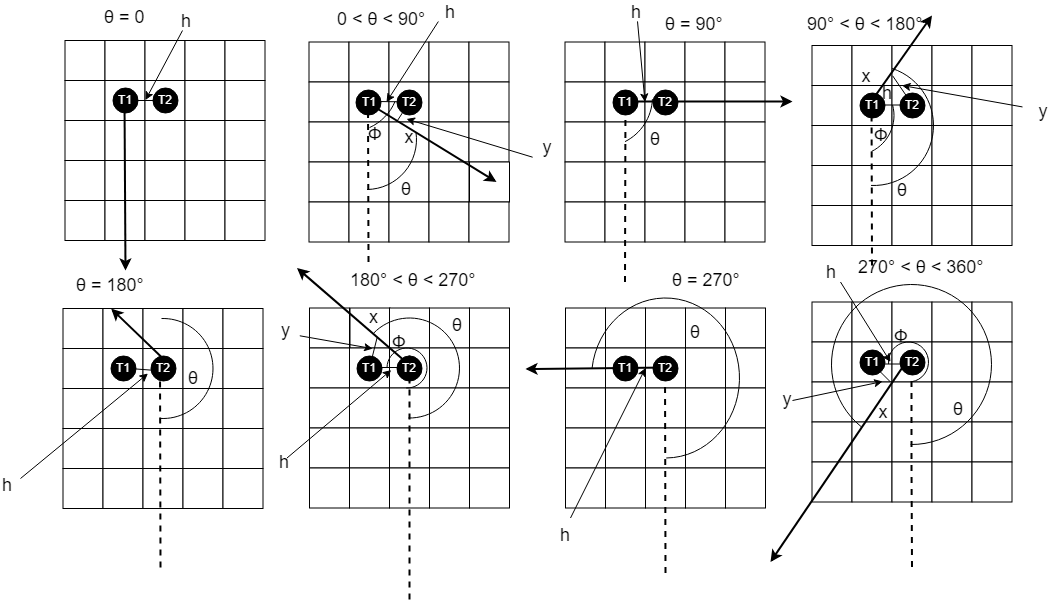
\includegraphics[width=\linewidth]{Figures/worstSmall.png}
            \caption{Schematics of a worst configuration of a 1km by 1km wind farm with two wind turbines located at $(1,1)$ and $(1,2)$ for different wind directions.}
            \label{worstSmall}
        \end{figure}
        
        Consider an example shown in Figure \ref{worstSmall} where the wind turbines $T_1$ and $T_2$ are located at $(1,1)$ and $(1,2)$ respectively with wind speed of $12m/s$ for every direction, the shortest distance between them $h$ is
        \begin{align*}
            h
            &=200m\cdot \sqrt{(1-1)^2 + (1-2)^2} \\
            &=200\;meters
        \end{align*}
        
        For wind directions $\theta=0^o$ as shown in Figure \ref{worstSmall}, the distance the two wind turbines with respect to the wind speed is $x=0$ while $y$ would be the same as $h$ by inspecting the figure. However, using our formula for x and y, the values would be the same as shown below.
        \begin{align*}
            \phi
        	&= tan^{-1} \left| \frac{1-2}{1-1} \right| \\
        	&= \lim_{\delta -> 0} \left( tan^{-1} \frac{1}{\delta} \right) \\
        	&= 90^o
        \end{align*}
            \begin{align*}
            x &= h(cos|(\theta\;mod\;90^{o})-\phi|) \\
              &= 200m(cos|0^{o}-90^{o}|) \\
              &= (200m)(0) \\
            x &= 0\;meters
        \end{align*}
    and the $y$ is
        \begin{align*}
            y &= h(sin|(\theta\;mod\;90^{o})-\phi|) \\
              &= 200m(cos|0^{o}-90^{o}|) \\
              &= (200m)(1) \\
            y &= 200\;meters
        \end{align*}
        
        The resulting radius of the wake at a distance of $x=0\;meters$ would be
        \begin{align*}
            r(x=0)&=(0.3267949)(0) + 20m \\
            &= 20 \;meters
        \end{align*}
        which is less than $y$ which implies that there is no wake interaction between the two wind turbines at that wind direction. Therefore, the power output of each wind turbine $P_1$ and $P_2$ is
        \begin{align*}
            P_1=P_2
            &=0.3(12m/s)^3 \\
            &= 518.4kW
        \end{align*}
        
        The summary of the computation of $x$, $y$, the resulting radius of the wake $r$, wind speed at each wind turbine $u_1$ $u_1$, and the power output of each wind turbine $P_1$ $P_1$ for the given worst configuration of the wind farm with two wind turbines are shown in Table \ref{summaryWorst2}.
        
        \singlespacing
    \begin{table}[H]
        \centering
        \begin{tabular}{|c|c|c|c|c|c|c|c|c|} \hline
    $\theta$ &$x$ &$y$ &$r$ &$u_1$ &$u_2$ &$P_1$ &$P_2$ &$P_1+P_2$ \\ \hline
$0^o$	&0.000	&200.000	&20.000	&12.000	&12.000	&518.400	&518.400	&1036.800 \\ \hline
$10^o$	&34.730	&196.962	&31.349	&12.000	&12.000	&518.400	&518.400	&1036.800 \\ \hline
$20^o$	&68.404	&187.939	&42.354	&12.000	&12.000	&518.400	&518.400	&1036.800 \\ \hline
$30^o$	&100.000	&173.205	&52.679	&12.000	&12.000	&518.400	&518.400	&1036.800 \\ \hline
$40^o$	&128.558	&153.209	&62.012	&12.000	&12.000	&518.400	&518.400	&1036.800 \\ \hline
$50^o$	&153.209	&128.558	&70.068	&12.000	&12.000	&518.400	&518.400	&1036.800 \\ \hline
$60^o$	&173.205	&100.000	&76.603	&12.000	&12.000	&518.400	&518.400	&1036.800 \\ \hline
$70^o$	&187.939	&68.404	&81.417	&12.000	&9.070	&518.400	&223.849	&742.249 \\ \hline
$80^o$	&196.962	&34.730	&84.366	&12.000	&9.176	&518.400	&231.819	&750.219 \\ \hline
$90^o$	&200.000	&0.000	&85.359	&12.000	&9.211	&518.400	&234.445	&752.845 \\ \hline
$100^o$	&34.730	&196.962	&31.349	&12.000	&12.000	&518.400	&518.400	&1036.800 \\ \hline
$110^o$	&68.404	&187.939	&42.354	&12.000	&12.000	&518.400	&518.400	&1036.800 \\ \hline
$120^o$	&100.000	&173.205	&52.679	&12.000	&12.000	&518.400	&518.400	&1036.800 \\ \hline
$130^o$	&128.558	&153.209	&62.012	&12.000	&12.000	&518.400	&518.400	&1036.800 \\ \hline
$140^o$	&153.209	&128.558	&70.068	&12.000	&12.000	&518.400	&518.400	&1036.800 \\ \hline
$150^o$	&173.205	&100.000	&76.603	&12.000	&12.000	&518.400	&518.400	&1036.800 \\ \hline
$160^o$	&187.939	&68.404	&81.417	&12.000	&9.070	&518.400	&223.849	&742.249 \\ \hline
$170^o$	&196.962	&34.730	&84.366	&12.000	&9.176	&518.400	&231.819	&750.219 \\ \hline
$180^o$	&0.000	&200.000	&20.000	&12.000	&12.000	&518.400	&518.400	&1036.800 \\ \hline
$190^o$	&34.730	&196.962	&31.349	&12.000	&12.000	&518.400	&518.400	&1036.800 \\ \hline
$200^o$	&68.404	&187.939	&42.354	&12.000	&12.000	&518.400	&518.400	&1036.800 \\ \hline
$210^o$	&100.000	&173.205	&52.679	&12.000	&12.000	&518.400	&518.400	&1036.800 \\ \hline
$220^o$	&128.558	&153.209	&62.012	&12.000	&12.000	&518.400	&518.400	&1036.800 \\ \hline
$230^o$	&153.209	&128.558	&70.068	&12.000	&12.000	&518.400	&518.400	&1036.800 \\ \hline
$240^o$	&173.205	&100.000	&76.603	&12.000	&12.000	&518.400	&518.400	&1036.800 \\ \hline
$250^o$	&187.939	&68.404	&81.417	&9.070	&12.000	&223.849	&518.400	&742.249 \\ \hline
$260^o$	&196.962	&34.730	&84.366	&9.176	&12.000	&231.819	&518.400	&750.219 \\ \hline
$270^o$	&200.000	&0.000	&85.359	&9.211	&12.000	&234.445	&518.400	&752.845 \\ \hline
$280^o$	&34.730	&196.962	&31.349	&12.000	&12.000	&518.400	&518.400	&1036.800 \\ \hline
$290^o$	&68.404	&187.939	&42.354	&12.000	&12.000	&518.400	&518.400	&1036.800 \\ \hline
$300^o$	&100.000	&173.205	&52.679	&12.000	&12.000	&518.400	&518.400	&1036.800 \\ \hline
$310^o$	&128.558	&153.209	&62.012	&12.000	&12.000	&518.400	&518.400	&1036.800 \\ \hline
$320^o$	&153.209	&128.558	&70.068	&12.000	&12.000	&518.400	&518.400	&1036.800 \\ \hline
$330^o$	&173.205	&100.000	&76.603	&12.000	&12.000	&518.400	&518.400	&1036.800 \\ \hline
$340^o$	&187.939	&68.404	&81.417	&9.070	&12.000	&223.849	&518.400	&742.249 \\ \hline
$350^o$	&196.962	&34.730	&84.366	&9.176	&12.000	&231.819	&518.400	&750.219 \\ \hline
        \end{tabular}
        \caption{Summary of the computation of $x$ (in meters), $y$ (in meters), the resulting radius of the wake $r$ (in meters), wind speed at each wind turbine $u_1$ $u_1$ (in m/s), the power output of each wind turbine $P_1$ $P_1$ (in kiloWatts) of two wind turbines located at $(1,1)$ and $(1,2)$ respectively on a 1km by 1km wind farm, and the total power output of the whole wind farm (in kiloWatts).}
        \label{summaryWorst2}
    \end{table}
    \doublespacing
    
    Since each wind direction's existence throughout the year is even, the fraction of occurrence of each wind direction is $\frac{1}{36}$. Therefore, the total annual power output of the whole wind farm with the current configuration would be
    \begin{align*}
        P_{tot}
        &= \sum_{\theta=0^o}^{350^o} \left( P_{1[\theta]} + P_{2[\theta]} \right) \cdot \frac{1}{36} \\
        &= \frac{1}{36}\left( P_{1[\theta=0^o]} + P_{2[\theta=0^o]} \right) + \frac{1}{36}\left( P_{1[\theta=10^o]} + P_{2[\theta=10^o]} \right) +...+ \frac{1}{36}\left( P_{1[\theta=350^o]} + P_{2[\theta=350^o]} \right) \\
        &= \frac{1}{36}\cdot\left( 518.4kW + 518.4kW \right) + \frac{1}{36}\cdot\left( 518.4kW + 518.4kW \right) +...+ \frac{1}{36}\cdot\left( 518.4kW + 281.8kW \right) \\
        &=956.4545kW
    \end{align*}
    
%%%%%%%%%%%%%%%%%ADDEDNDUM
\subsection{Power Output of Wind Turbines Located at (1,1) and (2,3)}  
    To justify if the previous configuration is indeed one of the worst configurations of two wind turbines, it is needed to take a look what will happen if the distance between the two wind turbines is increased. consider the same wind farm but where the wind turbine $T_2$ moved to location $(2,3)$. The distance between the two wind turbines $T_1$ and $T_2$ is
 
\begin{align*}
	h
	&=(200m)\sqrt{(1-2)^2+(1-3)^2} \\
	&=(200m)(2.23607) \\
	&=447.214\;meters
\end{align*}
and the angle between the references axis and the line connecting the two wind turbines is
\begin{align*}
	\phi
	&=tan^{-1}\left| \frac{(1-3)}{(1-2)} \right| \\
	&=tan^{-1} 2.000 \\
	&=63.435^o
\end{align*}

    \begin{figure}[H]
        \centering
        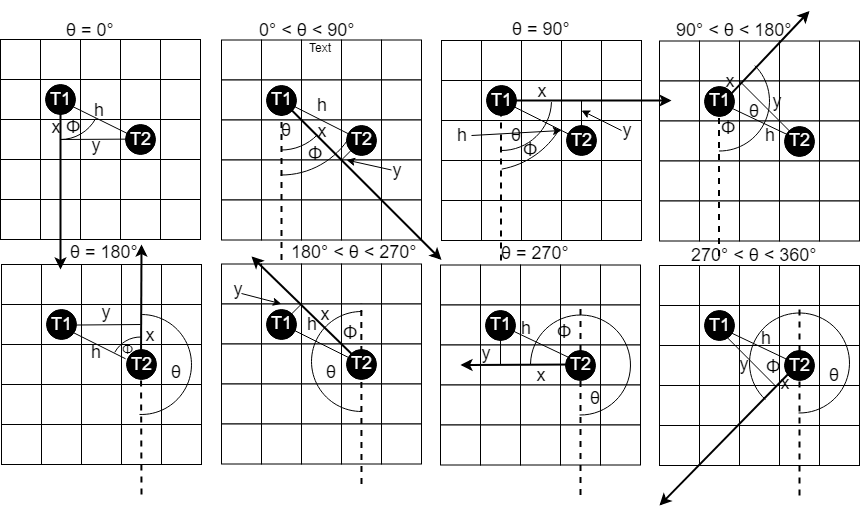
\includegraphics[width=\linewidth]{Figures/1123.png}
        \caption{Schematics of a worst configuration of a 1km by 1km wind farm with two wind turbines located at $(1,1)$ and $(2,3)$ for different wind directions.}
        \label{sampleSmall4}
    \end{figure}
    
    The manual computation of line segments $x$, $y$ from Figure \ref{sampleSmall4} and the resulting radius of the wake $r$ are shown below. If for the any wind direction where the resulting radius $r$ of the wake at a distance of $x$ is less than the length of $y$, then the wind speed of both wind turbines is both $u_1=u_2=12m/s$ and the power output of each is $P_1=P_2=518.400kW$.

    \begin{itemize}
\item $\theta=0^o$
	\begin{align*}%THETA=0
		x_{[\theta=0^o]} &=(447.214m) cos\left| (0^o\%90^o) - 63.435^o \right|  =199.1\;meters \\
		y_{[\theta=0^o]} &=(447.214m) sin\left| (0^o\%90^o) - 63.435^o \right|  =400.1\;meters \\
		r(199.1m) &=(0.32679491924311227)(199.1m)+20m  =85.65\;meters\end{align*}
\item $\theta=10^o$
	\begin{align*}%THETA=10
		x_{[\theta=10^o]} &=(447.214m) cos\left| (10^o\%90^o) - 63.435^o \right|  =266.421\;meters \\
		y_{[\theta=10^o]} &=(447.214m) sin\left| (10^o\%90^o) - 63.435^o \right|  =359.194\;meters \\
		r(266.421m) &=(0.32679491924311227)(266.421m)+20m  =107.065\;meters\end{align*}
\item $\theta=20^o$
	\begin{align*}%THETA=20
		x_{[\theta=20^o]} &=(447.214m) cos\left| (20^o\%90^o) - 63.435^o \right|  =324.747\;meters \\
		y_{[\theta=20^o]} &=(447.214m) sin\left| (20^o\%90^o) - 63.435^o \right|  =307.474\;meters \\
		r(324.747m) &=(0.32679491924311227)(324.747m)+20m  =126.126\;meters\end{align*}
\item $\theta=30^o$
	\begin{align*}%THETA=30
		x_{[\theta=30^o]} &=(447.214m) cos\left| (30^o\%90^o) - 63.435^o \right|  =373.205\;meters \\
		y_{[\theta=30^o]} &=(447.214m) sin\left| (30^o\%90^o) - 63.435^o \right|  =246.411\;meters \\
		r(373.205m) &=(0.32679491924311227)(373.205m)+20m  =141.961\;meters\end{align*}
\item $\theta=40^o$
	\begin{align*}%THETA=40
		x_{[\theta=40^o]} &=(447.214m) cos\left| (40^o\%90^o) - 63.435^o \right|  =410.324\;meters \\
		y_{[\theta=40^o]} &=(447.214m) sin\left| (40^o\%90^o) - 63.435^o \right|  =177.861\;meters \\
		r(410.324m) &=(0.32679491924311227)(410.324m)+20m  =154.92\;meters\end{align*}
\item $\theta=50^o$
	\begin{align*}%THETA=50
		x_{[\theta=50^o]} &=(447.214m) cos\left| (50^o\%90^o) - 63.435^o \right|  =434.976\;meters \\
		y_{[\theta=50^o]} &=(447.214m) sin\left| (50^o\%90^o) - 63.435^o \right|  =103.907\;meters \\
		r(434.976m) &=(0.32679491924311227)(434.976m)+20m  =162.148\;meters\\
		u_{2[\theta=50^o]} &=(12m/s)\left( 1-2(0.326795)\left( \frac{27.881}{27.881+(0.9437)(434.976m)} \right)^2 \right) =10.717\;m/s \\
		P_{2[\theta=50^o]} &=0.3(10.717m/s)^3  =369.267\;kiloWatts
\end{align*}
\item $\theta=60^o$
	\begin{align*}%THETA=60
		x_{[\theta=60^o]} &=(447.214m) cos\left| (60^o\%90^o) - 63.435^o \right|  =446.411\;meters \\
		y_{[\theta=60^o]} &=(447.214m) sin\left| (60^o\%90^o) - 63.435^o \right|  =26.795\;meters \\
		r(446.411m) &=(0.32679491924311227)(446.411m)+20m  =165.885\;meters\\
		u_{2[\theta=60^o]} &=(12m/s)\left( 1-2(0.326795)\left( \frac{27.881}{27.881+(0.9437)(446.411m)} \right)^2 \right) =10.756\;m/s \\
		P_{2[\theta=60^o]} &=0.3(10.756m/s)^3  =373.313\;kiloWatts
\end{align*}
\item $\theta=70^o$
	\begin{align*}%THETA=70
		x_{[\theta=70^o]} &=(447.214m) cos\left| (70^o\%90^o) - 63.435^o \right|  =444.282\;meters \\
		y_{[\theta=70^o]} &=(447.214m) sin\left| (70^o\%90^o) - 63.435^o \right|  =51.13\;meters \\
		r(444.282m) &=(0.32679491924311227)(444.282m)+20m  =165.189\;meters\\
		u_{2[\theta=70^o]} &=(12m/s)\left( 1-2(0.326795)\left( \frac{27.881}{27.881+(0.9437)(444.282m)} \right)^2 \right) =10.749\;m/s \\
		P_{2[\theta=70^o]} &=0.3(10.749m/s)^3  =372.585\;kiloWatts
\end{align*}
\item $\theta=80^o$
	\begin{align*}%THETA=80
		x_{[\theta=80^o]} &=(447.214m) cos\left| (80^o\%90^o) - 63.435^o \right|  =428.653\;meters \\
		y_{[\theta=80^o]} &=(447.214m) sin\left| (80^o\%90^o) - 63.435^o \right|  =127.502\;meters \\
		r(428.653m) &=(0.32679491924311227)(428.653m)+20m  =160.82\;meters\\
		u_{2[\theta=80^o]} &=(12m/s)\left( 1-2(0.326795)\left( \frac{27.881}{27.881+(0.9437)(428.653m)} \right)^2 \right) =10.694\;m/s \\
		P_{2[\theta=80^o]} &=0.3(10.694m/s)^3  =366.895\;kiloWatts
\end{align*}
\item $\theta=90^o$
	\begin{align*}%THETA=90
		x_{[\theta=90^o]} &=(447.214m) cos\left| 90^o - 63.435^o \right|  =400.1\;meters \\
		y_{[\theta=90^o]} &=(447.214m) sin\left| 90^o - 63.435^o \right|  =199.1\;meters \\
		r(400.1m) &=(0.32679491924311227)(400.1m)+20m  =150.751\;meters\end{align*}
\item $\theta=100^o$
	\begin{align*}%THETA=100
		x_{[\theta=100^o]} &=(447.214m) cos\left| (100^o\%90^o) - 63.435^o \right|  =266.421\;meters \\
		y_{[\theta=100^o]} &=(447.214m) sin\left| (100^o\%90^o) - 63.435^o \right|  =359.194\;meters \\
		r(266.421m) &=(0.32679491924311227)(266.421m)+20m  =107.065\;meters\end{align*}
\item $\theta=110^o$
	\begin{align*}%THETA=110
		x_{[\theta=110^o]} &=(447.214m) cos\left| (110^o\%90^o) - 63.435^o \right|  =324.747\;meters \\
		y_{[\theta=110^o]} &=(447.214m) sin\left| (110^o\%90^o) - 63.435^o \right|  =307.474\;meters \\
		r(324.747m) &=(0.32679491924311227)(324.747m)+20m  =126.126\;meters\end{align*}
\item $\theta=120^o$
	\begin{align*}%THETA=120
		x_{[\theta=120^o]} &=(447.214m) cos\left| (120^o\%90^o) - 63.435^o \right|  =373.205\;meters \\
		y_{[\theta=120^o]} &=(447.214m) sin\left| (120^o\%90^o) - 63.435^o \right|  =246.411\;meters \\
		r(373.205m) &=(0.32679491924311227)(373.205m)+20m  =141.961\;meters\end{align*}
\item $\theta=130^o$
	\begin{align*}%THETA=130
		x_{[\theta=130^o]} &=(447.214m) cos\left| (130^o\%90^o) - 63.435^o \right|  =410.324\;meters \\
		y_{[\theta=130^o]} &=(447.214m) sin\left| (130^o\%90^o) - 63.435^o \right|  =177.861\;meters \\
		r(410.324m) &=(0.32679491924311227)(410.324m)+20m  =154.92\;meters\end{align*}
\item $\theta=140^o$
	\begin{align*}%THETA=140
		x_{[\theta=140^o]} &=(447.214m) cos\left| (140^o\%90^o) - 63.435^o \right|  =434.976\;meters \\
		y_{[\theta=140^o]} &=(447.214m) sin\left| (140^o\%90^o) - 63.435^o \right|  =103.907\;meters \\
		r(434.976m) &=(0.32679491924311227)(434.976m)+20m  =162.148\;meters\end{align*}
\item $\theta=150^o$
	\begin{align*}%THETA=150
		x_{[\theta=150^o]} &=(447.214m) cos\left| (150^o\%90^o) - 63.435^o \right|  =446.411\;meters \\
		y_{[\theta=150^o]} &=(447.214m) sin\left| (150^o\%90^o) - 63.435^o \right|  =26.795\;meters \\
		r(446.411m) &=(0.32679491924311227)(446.411m)+20m  =165.885\;meters\end{align*}
\item $\theta=160^o$
	\begin{align*}%THETA=160
		x_{[\theta=160^o]} &=(447.214m) cos\left| (160^o\%90^o) - 63.435^o \right|  =444.282\;meters \\
		y_{[\theta=160^o]} &=(447.214m) sin\left| (160^o\%90^o) - 63.435^o \right|  =51.13\;meters \\
		r(444.282m) &=(0.32679491924311227)(444.282m)+20m  =165.189\;meters\end{align*}
\item $\theta=170^o$
	\begin{align*}%THETA=170
		x_{[\theta=170^o]} &=(447.214m) cos\left| (170^o\%90^o) - 63.435^o \right|  =428.653\;meters \\
		y_{[\theta=170^o]} &=(447.214m) sin\left| (170^o\%90^o) - 63.435^o \right|  =127.502\;meters \\
		r(428.653m) &=(0.32679491924311227)(428.653m)+20m  =160.82\;meters\end{align*}
    \end{itemize}

    For the rest of the wind directions ($180^o\leq \theta<360^o$), the power output of each wind wind turbines should interchange for opposite angles. For instance, the power output $P_{1[\theta=50^o]}$ and $P_{2[\theta=50^o]}$ of the wind turbines would be the same as the power output $P_{2[\theta=230^o]}$ and $P_{1[\theta=230^o]}$, respectively. That is,
    \begin{align*}
        P_{1[\theta=50^o]} = P_{2[\theta=230^o]} = 369.267\;kiloWatts \\
        P_{2[\theta=50^o]} = P_{1[\theta=230^o]} = 518.400\;kiloWatts
    \end{align*}
    
    The same computations were made using a computer and the computed values are shown in Table \ref{summaryAvg1}. Since each wind direction's existence throughout the year is even, the fraction of occurrence of each wind direction is $\frac{1}{36}$. Therefore, the total annual power output of the whole wind farm with the current configuration would be
    
    %T1: (1,1) T2: (2,3)
    %h: 447.2131 phi: 63.4341   p_tot = 1003.9369108556124
    \singlespacing
    \begin{table}[H]
        \centering
        \begin{tabular}{|c|c|c|c|c|c|c|c|c|} \hline
    $\theta$ &$x$ &$y$ &$r$ &$u_1$ &$u_2$ &$P_1$ &$P_2$ &$P_1+P_2$ \\ \hline
$0^o$	&200.000	&400.000	&85.359	&12.000	&12.000	&518.400	&518.400	&1036.800 \\ \hline
$10^o$	&266.421	&359.193	&107.065	&12.000	&12.000	&518.400	&518.400	&1036.800 \\ \hline
$20^o$	&324.747	&307.473	&126.126	&12.000	&12.000	&518.400	&518.400	&1036.800 \\ \hline
$30^o$	&373.205	&246.410	&141.962	&12.000	&12.000	&518.400	&518.400	&1036.800 \\ \hline
$40^o$	&410.324	&177.860	&154.092	&12.000	&12.000	&518.400	&518.400	&1036.800 \\ \hline
$50^o$	&434.975	&103.906	&162.148	&12.000	&10.717	&518.400	&369.247	&887.647 \\ \hline
$60^o$	&446.410	&26.795	&165.885	&12.000	&10.756	&518.400	&373.319	&891.719 \\ \hline
$70^o$	&444.281	&51.130	&165.189	&12.000	&10.749	&518.400	&372.573	&890.973 \\ \hline
$80^o$	&428.653	&127.502	&160.082	&12.000	&10.694	&518.400	&366.925	&885.325 \\ \hline
$90^o$	&400.000	&200.000	&150.718	&12.000	&12.000	&518.400	&518.400	&1036.800 \\ \hline
$100^o$	&266.421	&359.193	&107.065	&12.000	&12.000	&518.400	&518.400	&1036.800 \\ \hline
$110^o$	&324.747	&307.473	&126.126	&12.000	&12.000	&518.400	&518.400	&1036.800 \\ \hline
$120^o$	&373.205	&246.410	&141.962	&12.000	&12.000	&518.400	&518.400	&1036.800 \\ \hline
$130^o$	&410.324	&177.860	&154.092	&12.000	&12.000	&518.400	&518.400	&1036.800 \\ \hline
$140^o$	&434.975	&103.906	&162.148	&12.000	&12.000	&518.400	&518.400	&1036.800 \\ \hline
$150^o$	&446.410	&26.795	&165.885	&12.000	&12.000	&518.400	&518.400	&1036.800 \\ \hline
$160^o$	&444.281	&51.130	&165.189	&12.000	&12.000	&518.400	&518.400	&1036.800 \\ \hline
$170^o$	&428.653	&127.502	&160.082	&12.000	&12.000	&518.400	&518.400	&1036.800 \\ \hline
$180^o$	&200.000	&400.000	&85.359	&12.000	&12.000	&518.400	&518.400	&1036.800 \\ \hline
$190^o$	&266.421	&359.193	&107.065	&12.000	&12.000	&518.400	&518.400	&1036.800 \\ \hline
$200^o$	&324.747	&307.473	&126.126	&12.000	&12.000	&518.400	&518.400	&1036.800 \\ \hline
$210^o$	&373.205	&246.410	&141.962	&12.000	&12.000	&518.400	&518.400	&1036.800 \\ \hline
$220^o$	&410.324	&177.860	&154.092	&12.000	&12.000	&518.400	&518.400	&1036.800 \\ \hline
$230^o$	&434.975	&103.906	&162.148	&10.717	&12.000	&369.247	&518.400	&887.647 \\ \hline
$240^o$	&446.410	&26.795	&165.885	&10.756	&12.000	&373.319	&518.400	&891.719 \\ \hline
$250^o$	&444.281	&51.130	&165.189	&10.749	&12.000	&372.573	&518.400	&890.973 \\ \hline
$260^o$	&428.653	&127.502	&160.082	&10.694	&12.000	&366.925	&518.400	&885.325 \\ \hline
$270^o$	&400.000	&200.000	&150.718	&12.000	&12.000	&518.400	&518.400	&1036.800 \\ \hline
$280^o$	&266.421	&359.193	&107.065	&12.000	&12.000	&518.400	&518.400	&1036.800 \\ \hline
$290^o$	&324.747	&307.473	&126.126	&12.000	&12.000	&518.400	&518.400	&1036.800 \\ \hline
$300^o$	&373.205	&246.410	&141.962	&12.000	&12.000	&518.400	&518.400	&1036.800 \\ \hline
$310^o$	&410.324	&177.860	&154.092	&12.000	&12.000	&518.400	&518.400	&1036.800 \\ \hline
$320^o$	&434.975	&103.906	&162.148	&12.000	&12.000	&518.400	&518.400	&1036.800 \\ \hline
$330^o$	&446.410	&26.795	&165.885	&12.000	&12.000	&518.400	&518.400	&1036.800 \\ \hline
$340^o$	&444.281	&51.130	&165.189	&12.000	&12.000	&518.400	&518.400	&1036.800 \\ \hline
$350^o$	&428.653	&127.502	&160.082	&12.000	&12.000	&518.400	&518.400	&1036.800 \\ \hline
        \end{tabular}
        \caption{Summary of the computation of $x$ (in meters), $y$ (in meters), the resulting radius of the wake $r$ (in meters), wind speed at each wind turbine $u_1$ $u_1$ (in m/s), the power output of each wind turbine $P_1$ $P_1$ (in kiloWatts) of two wind turbines located at $(1,1)$ and $(2,3)$ respectively on a 1km by 1km wind farm, and the total power output of the whole wind farm (in kiloWatts).}
        \label{summaryAvg1}
    \end{table}
    \doublespacing
    
    \begin{align*}
        P_{tot}
        &= \sum_{\theta=0^o}^{350^o} \left( P_{1[\theta]} + P_{2[\theta]} \right) \cdot \frac{1}{36} \\
        &= \frac{1}{36}\left( P_{1[\theta=0^o]} + P_{2[\theta=0^o]} \right) + \frac{1}{36}\left( P_{1[\theta=10^o]} + P_{2[\theta=10^o]} \right) +...+ \frac{1}{36}\left( P_{1[\theta=350^o]} + P_{2[\theta=350^o]} \right) \\
        &= \frac{1}{36}\cdot\left( 518.4kW + 518.4kW \right) + \frac{1}{36}\cdot\left( 518.4kW + 518.4kW \right) +...+ \frac{1}{36}\cdot\left(  518.4kW + 518.4kW \right) \\
        &=1003.937\;kiloWatts
    \end{align*}
    
\subsection{Power Output of Wind Turbines Located at (1,3) and (3,2)}   
    Consider another configuration but with the same distance of $h=447.214\;meters$ between the wind turbines as with the previous configuration. The locations of the wind turbines $T_1$ and $T_2$ are $(1,3)$ and $(3,2)$ respectively. The angle between the the reference axis and the line connecting the two wind turbines as labelled as $\phi$ in Figure \ref{sampleSmall5} is
    \begin{align*}
    	\phi
    	&=tan^{-1}\left| \frac{(3-2)}{(1-3)} \right| \\
    	&=tan^{-1} 0.500 \\
    	&=26.565^o
    \end{align*}
    
    The manual computation of line segments $x$, $y$ from Figure \ref{sampleSmall5} and the resulting radius of the wake $r$ are shown below. If for the any wind direction where the resulting radius $r$ of the wake at a distance of $x$ is less than the length of $y$, then the wind speed of both wind turbines is both $u_1=u_2=12m/s$ and the power output of each is $P_1=P_2=518.400kW$.
    
    \begin{figure}[H]
        \centering
        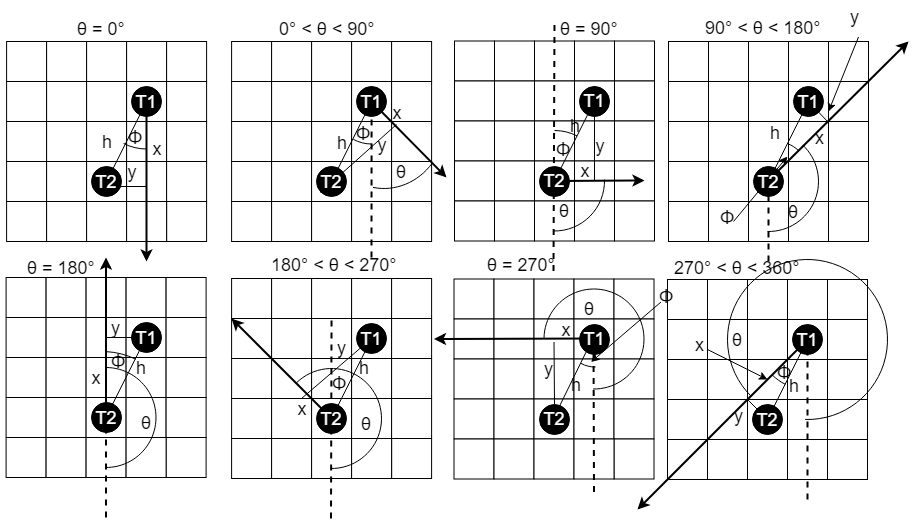
\includegraphics[width=\linewidth]{Figures/1332.png}
        \caption{Schematics of a worst configuration of a 1km by 1km wind farm with two wind turbines located at $(1,3)$ and $(3,2)$ for different wind directions.}
        \label{sampleSmall5}
    \end{figure}
    
    \begin{itemize}
\item $\theta=0^o$
	\begin{align*}%THETA=0
		x_{[\theta=0^o]} &=(447.214m) cos\left| (0^o\%90^o) - 26.565^o \right|  =400.1\;meters \\
		y_{[\theta=0^o]} &=(447.214m) sin\left| (0^o\%90^o) - 26.565^o \right|  =199.1\;meters \\
		r(400.1m) &=(0.32679491924311227)(400.1m)+20m  =150.751\;meters\end{align*}
\item $\theta=10^o$
	\begin{align*}%THETA=10
		x_{[\theta=10^o]} &=(447.214m) cos\left| (10^o\%90^o) - 26.565^o \right|  =428.653\;meters \\
		y_{[\theta=10^o]} &=(447.214m) sin\left| (10^o\%90^o) - 26.565^o \right|  =127.502\;meters \\
		r(428.653m) &=(0.32679491924311227)(428.653m)+20m  =160.82\;meters\end{align*}
\item $\theta=20^o$
	\begin{align*}%THETA=20
		x_{[\theta=20^o]} &=(447.214m) cos\left| (20^o\%90^o) - 26.565^o \right|  =444.282\;meters \\
		y_{[\theta=20^o]} &=(447.214m) sin\left| (20^o\%90^o) - 26.565^o \right|  =51.13\;meters \\
		r(444.282m) &=(0.32679491924311227)(444.282m)+20m  =165.189\;meters\end{align*}
\item $\theta=30^o$
	\begin{align*}%THETA=30
		x_{[\theta=30^o]} &=(447.214m) cos\left| (30^o\%90^o) - 26.565^o \right|  =446.411\;meters \\
		y_{[\theta=30^o]} &=(447.214m) sin\left| (30^o\%90^o) - 26.565^o \right|  =26.795\;meters \\
		r(446.411m) &=(0.32679491924311227)(446.411m)+20m  =165.885\;meters\end{align*}
\item $\theta=40^o$
	\begin{align*}%THETA=40
		x_{[\theta=40^o]} &=(447.214m) cos\left| (40^o\%90^o) - 26.565^o \right|  =434.976\;meters \\
		y_{[\theta=40^o]} &=(447.214m) sin\left| (40^o\%90^o) - 26.565^o \right|  =103.907\;meters \\
		r(434.976m) &=(0.32679491924311227)(434.976m)+20m  =162.148\;meters\end{align*}
\item $\theta=50^o$
	\begin{align*}%THETA=50
		x_{[\theta=50^o]} &=(447.214m) cos\left| (50^o\%90^o) - 26.565^o \right|  =410.324\;meters \\
		y_{[\theta=50^o]} &=(447.214m) sin\left| (50^o\%90^o) - 26.565^o \right|  =177.861\;meters \\
		r(410.324m) &=(0.32679491924311227)(410.324m)+20m  =154.92\;meters\end{align*}
\item $\theta=60^o$
	\begin{align*}%THETA=60
		x_{[\theta=60^o]} &=(447.214m) cos\left| (60^o\%90^o) - 26.565^o \right|  =373.205\;meters \\
		y_{[\theta=60^o]} &=(447.214m) sin\left| (60^o\%90^o) - 26.565^o \right|  =246.411\;meters \\
		r(373.205m) &=(0.32679491924311227)(373.205m)+20m  =141.961\;meters\end{align*}
\item $\theta=70^o$
	\begin{align*}%THETA=70
		x_{[\theta=70^o]} &=(447.214m) cos\left| (70^o\%90^o) - 26.565^o \right|  =324.747\;meters \\
		y_{[\theta=70^o]} &=(447.214m) sin\left| (70^o\%90^o) - 26.565^o \right|  =307.474\;meters \\
		r(324.747m) &=(0.32679491924311227)(324.747m)+20m  =126.126\;meters\end{align*}
\item $\theta=80^o$
	\begin{align*}%THETA=80
		x_{[\theta=80^o]} &=(447.214m) cos\left| (80^o\%90^o) - 26.565^o \right|  =266.421\;meters \\
		y_{[\theta=80^o]} &=(447.214m) sin\left| (80^o\%90^o) - 26.565^o \right|  =359.194\;meters \\
		r(266.421m) &=(0.32679491924311227)(266.421m)+20m  =107.065\;meters\end{align*}
\item $\theta=90^o$
	\begin{align*}%THETA=90
		x_{[\theta=90^o]} &=(447.214m) cos\left| 90^o - 26.565^o \right|  =199.1\;meters \\
		y_{[\theta=90^o]} &=(447.214m) sin\left| 90^o - 26.565^o \right|  =400.1\;meters \\
		r(199.1m) &=(0.32679491924311227)(199.1m)+20m  =85.65\;meters\end{align*}
\item $\theta=100^o$
	\begin{align*}%THETA=100
		x_{[\theta=100^o]} &=(447.214m) cos\left| (100^o\%90^o) - 26.565^o \right|  =428.653\;meters \\
		y_{[\theta=100^o]} &=(447.214m) sin\left| (100^o\%90^o) - 26.565^o \right|  =127.502\;meters \\
		r(428.653m) &=(0.32679491924311227)(428.653m)+20m  =160.82\;meters\\
		u_{1[\theta=100^o]} &=(12m/s)\left( 1-2(0.326795)\left( \frac{27.881}{27.881+(0.9437)(428.653m)} \right)^2 \right) =10.694\;m/s \\
		P_{1[\theta=100^o]} &=0.3(10.694m/s)^3  =366.895\;kiloWatts
\end{align*}
\item $\theta=110^o$
	\begin{align*}%THETA=110
		x_{[\theta=110^o]} &=(447.214m) cos\left| (110^o\%90^o) - 26.565^o \right|  =444.282\;meters \\
		y_{[\theta=110^o]} &=(447.214m) sin\left| (110^o\%90^o) - 26.565^o \right|  =51.13\;meters \\
		r(444.282m) &=(0.32679491924311227)(444.282m)+20m  =165.189\;meters\\
		u_{1[\theta=110^o]} &=(12m/s)\left( 1-2(0.326795)\left( \frac{27.881}{27.881+(0.9437)(444.282m)} \right)^2 \right) =10.749\;m/s \\
		P_{1[\theta=110^o]} &=0.3(10.749m/s)^3  =372.585\;kiloWatts
\end{align*}
\item $\theta=120^o$
	\begin{align*}%THETA=120
		x_{[\theta=120^o]} &=(447.214m) cos\left| (120^o\%90^o) - 26.565^o \right|  =446.411\;meters \\
		y_{[\theta=120^o]} &=(447.214m) sin\left| (120^o\%90^o) - 26.565^o \right|  =26.795\;meters \\
		r(446.411m) &=(0.32679491924311227)(446.411m)+20m  =165.885\;meters\\
		u_{1[\theta=120^o]} &=(12m/s)\left( 1-2(0.326795)\left( \frac{27.881}{27.881+(0.9437)(446.411m)} \right)^2 \right) =10.756\;m/s \\
		P_{1[\theta=120^o]} &=0.3(10.756m/s)^3  =373.313\;kiloWatts
\end{align*}
\item $\theta=130^o$
	\begin{align*}%THETA=130
		x_{[\theta=130^o]} &=(447.214m) cos\left| (130^o\%90^o) - 26.565^o \right|  =434.976\;meters \\
		y_{[\theta=130^o]} &=(447.214m) sin\left| (130^o\%90^o) - 26.565^o \right|  =103.907\;meters \\
		r(434.976m) &=(0.32679491924311227)(434.976m)+20m  =162.148\;meters\\
		u_{1[\theta=130^o]} &=(12m/s)\left( 1-2(0.326795)\left( \frac{27.881}{27.881+(0.9437)(434.976m)} \right)^2 \right) =10.717\;m/s \\
		P_{1[\theta=130^o]} &=0.3(10.717m/s)^3  =369.267\;kiloWatts
\end{align*}
\item $\theta=140^o$
	\begin{align*}%THETA=140
		x_{[\theta=140^o]} &=(447.214m) cos\left| (140^o\%90^o) - 26.565^o \right|  =410.324\;meters \\
		y_{[\theta=140^o]} &=(447.214m) sin\left| (140^o\%90^o) - 26.565^o \right|  =177.861\;meters \\
		r(410.324m) &=(0.32679491924311227)(410.324m)+20m  =154.92\;meters\end{align*}
\item $\theta=150^o$
	\begin{align*}%THETA=150
		x_{[\theta=150^o]} &=(447.214m) cos\left| (150^o\%90^o) - 26.565^o \right|  =373.205\;meters \\
		y_{[\theta=150^o]} &=(447.214m) sin\left| (150^o\%90^o) - 26.565^o \right|  =246.411\;meters \\
		r(373.205m) &=(0.32679491924311227)(373.205m)+20m  =141.961\;meters\end{align*}
\item $\theta=160^o$
	\begin{align*}%THETA=160
		x_{[\theta=160^o]} &=(447.214m) cos\left| (160^o\%90^o) - 26.565^o \right|  =324.747\;meters \\
		y_{[\theta=160^o]} &=(447.214m) sin\left| (160^o\%90^o) - 26.565^o \right|  =307.474\;meters \\
		r(324.747m) &=(0.32679491924311227)(324.747m)+20m  =126.126\;meters\end{align*}
\item $\theta=170^o$
	\begin{align*}%THETA=170
		x_{[\theta=170^o]} &=(447.214m) cos\left| (170^o\%90^o) - 26.565^o \right|  =266.421\;meters \\
		y_{[\theta=170^o]} &=(447.214m) sin\left| (170^o\%90^o) - 26.565^o \right|  =359.194\;meters \\
		r(266.421m) &=(0.32679491924311227)(266.421m)+20m  =107.065\;meters\end{align*}
    \end{itemize}
    
    For the rest of the wind directions ($180^o\leq \theta<360^o$), the power output of each wind wind turbines should interchange for opposite angles. For instance, the power output $P_{1[\theta=100^o]}$ and $P_{2[\theta=100^o]}$ of the wind turbines would be the same as the power output $P_{2[\theta=280^o]}$ and $P_{1[\theta=280^o]}$, respectively. That is,
    \begin{align*}
        P_{1[\theta=100^o]} = P_{2[\theta=280^o]} = 518.400\;kiloWatts \\
        P_{2[\theta=100^o]} = P_{1[\theta=280^o]} = 366.895\;kiloWatts
    \end{align*}
    
    The same computations were made using a computer and the computed values are shown in Table \ref{summaryAvg2}.
    
    %T1: (1,3) T2: (3,2)
    %h: 447.2131 phi: 0.0   p_tot = 1003.9369108556124
    \singlespacing
    \begin{table}[H]
        \centering
        \begin{tabular}{|c|c|c|c|c|c|c|c|c|} \hline
    $\theta$ &$x$ &$y$ &$r$ &$u_1$ &$u_2$ &$P_1$ &$P_2$ &$P_1+P_2$ \\ \hline
$0^o$	&400.000	&200.000	&150.718	&12.000	&12.000	&518.400	&518.400	&1036.800 \\ \hline
$10^o$	&428.653	&127.502	&160.082	&12.000	&12.000	&518.400	&518.400	&1036.800 \\ \hline
$20^o$	&444.281	&51.130	&165.189	&12.000	&12.000	&518.400	&518.400	&1036.800 \\ \hline
$30^o$	&446.410	&26.795	&165.885	&12.000	&12.000	&518.400	&518.400	&1036.800 \\ \hline
$40^o$	&434.975	&103.906	&162.148	&12.000	&12.000	&518.400	&518.400	&1036.800 \\ \hline
$50^o$	&410.324	&177.860	&154.092	&12.000	&12.000	&518.400	&518.400	&1036.800 \\ \hline
$60^o$	&373.205	&246.410	&141.962	&12.000	&12.000	&518.400	&518.400	&1036.800 \\ \hline
$70^o$	&324.747	&307.473	&126.126	&12.000	&12.000	&518.400	&518.400	&1036.800 \\ \hline
$80^o$	&266.421	&359.193	&107.065	&12.000	&12.000	&518.400	&518.400	&1036.800 \\ \hline
$90^o$	&200.000	&400.000	&85.359	&12.000	&12.000	&518.400	&518.400	&1036.800 \\ \hline
$100^o$	&428.653	&127.502	&160.082	&10.694	&12.000	&366.925	&518.400	&885.325 \\ \hline
$110^o$	&444.281	&51.130	&165.189	&10.749	&12.000	&372.573	&518.400	&890.973 \\ \hline
$120^o$	&446.410	&26.795	&165.885	&10.756	&12.000	&373.319	&518.400	&891.719 \\ \hline
$130^o$	&434.975	&103.906	&162.148	&10.717	&12.000	&369.247	&518.400	&887.647 \\ \hline
$140^o$	&410.324	&177.860	&154.092	&12.000	&12.000	&518.400	&518.400	&1036.800 \\ \hline
$150^o$	&373.205	&246.410	&141.962	&12.000	&12.000	&518.400	&518.400	&1036.800 \\ \hline
$160^o$	&324.747	&307.473	&126.126	&12.000	&12.000	&518.400	&518.400	&1036.800 \\ \hline
$170^o$	&266.421	&359.193	&107.065	&12.000	&12.000	&518.400	&518.400	&1036.800 \\ \hline
$180^o$	&400.000	&200.000	&150.718	&12.000	&12.000	&518.400	&518.400	&1036.800 \\ \hline
$190^o$	&428.653	&127.502	&160.082	&12.000	&12.000	&518.400	&518.400	&1036.800 \\ \hline
$200^o$	&444.281	&51.130	&165.189	&12.000	&12.000	&518.400	&518.400	&1036.800 \\ \hline
$210^o$	&446.410	&26.795	&165.885	&12.000	&12.000	&518.400	&518.400	&1036.800 \\ \hline
$220^o$	&434.975	&103.906	&162.148	&12.000	&12.000	&518.400	&518.400	&1036.800 \\ \hline
$230^o$	&410.324	&177.860	&154.092	&12.000	&12.000	&518.400	&518.400	&1036.800 \\ \hline
$240^o$	&373.205	&246.410	&141.962	&12.000	&12.000	&518.400	&518.400	&1036.800 \\ \hline
$250^o$	&324.747	&307.473	&126.126	&12.000	&12.000	&518.400	&518.400	&1036.800 \\ \hline
$260^o$	&266.421	&359.193	&107.065	&12.000	&12.000	&518.400	&518.400	&1036.800 \\ \hline
$270^o$	&200.000	&400.000	&85.359	&12.000	&12.000	&518.400	&518.400	&1036.800 \\ \hline
$280^o$	&428.653	&127.502	&160.082	&12.000	&10.694	&518.400	&366.925	&885.325 \\ \hline
$290^o$	&444.281	&51.130	&165.189	&12.000	&10.749	&518.400	&372.573	&890.973 \\ \hline
$300^o$	&446.410	&26.795	&165.885	&12.000	&10.756	&518.400	&373.319	&891.719 \\ \hline
$310^o$	&434.975	&103.906	&162.148	&12.000	&10.717	&518.400	&369.247	&887.647 \\ \hline
$320^o$	&410.324	&177.860	&154.092	&12.000	&12.000	&518.400	&518.400	&1036.800 \\ \hline
$330^o$	&373.205	&246.410	&141.962	&12.000	&12.000	&518.400	&518.400	&1036.800 \\ \hline
$340^o$	&324.747	&307.473	&126.126	&12.000	&12.000	&518.400	&518.400	&1036.800 \\ \hline
$350^o$	&266.421	&359.193	&107.065	&12.000	&12.000	&518.400	&518.400	&1036.800 \\ \hline
        \end{tabular}
        \caption{Summary of the computation of $x$ (in meters), $y$ (in meters), the resulting radius of the wake $r$ (in meters), wind speed at each wind turbine $u_1$ $u_1$ (in m/s), the power output of each wind turbine $P_1$ $P_1$ (in kiloWatts) of two wind turbines located at $(1,3)$ and $(3,2)$ respectively on a 1km by 1km wind farm, and the total power output of the whole wind farm (in kiloWatts).}
        \label{summaryAvg2}
    \end{table}
    \doublespacing
    
    Since each wind direction's existence throughout the year is even, the fraction of occurrence of each wind direction is $\frac{1}{36}$. Therefore, the total annual power output of the whole wind farm with the current configuration would be
    \begin{align*}
        P_{tot}
        &= \sum_{\theta=0^o}^{350^o} \left( P_{1[\theta]} + P_{2[\theta]} \right) \cdot \frac{1}{36} \\
        &= \frac{1}{36}\left( P_{1[\theta=0^o]} + P_{2[\theta=0^o]} \right) + \frac{1}{36}\left( P_{1[\theta=10^o]} + P_{2[\theta=10^o]} \right) +...+ \frac{1}{36}\left( P_{1[\theta=350^o]} + P_{2[\theta=350^o]} \right) \\
        &= \frac{1}{36}\cdot\left( 518.4kW + 518.4kW \right) + \frac{1}{36}\cdot\left( 518.4kW + 518.4kW \right) +...+ \frac{1}{36}\cdot\left(  518.4kW + 518.4kW \right) \\
        &=1003.937\;kiloWatts
    \end{align*}

\subsection{Power Output of Wind Turbines Located at (1,1) and (4,2)}   
    It is proven that from a worst configuration ($T_1(1,1); T_2(1,2)$), the total power output increases as the distance $h$ between the two wind turbines increases. To further support the claim, consider another configuration where the two wind turbines are farther from each other compared with the previous configuration with $h=447.214\;meters$. The location of the wind turbines $T_1$ and $T_2$ are $(1,1)$ and $(4,2)$ respectively. The distance between them is
    
    \begin{align*}
    	h
    	&=(200m)\sqrt{(1-4)^2+(1-2)^2} \\
    	&=(200m)(3.16228) \\
    	&=632.456\;meters
    \end{align*}
    which is higher than that of the previous configuration, and the angle between the reference line and the line connecting the two wind turbines labelled as $\phi$ in Figure \ref{sampleSmall6} is
    \begin{align*}
    	\phi
    	&=tan^{-1}\left| \frac{(1-2)}{(1-4)} \right| \\
    	&=tan^{-1} 0.333 \\
    	&=18.435^o
    \end{align*}
    
    \begin{figure}[H]
        \centering
        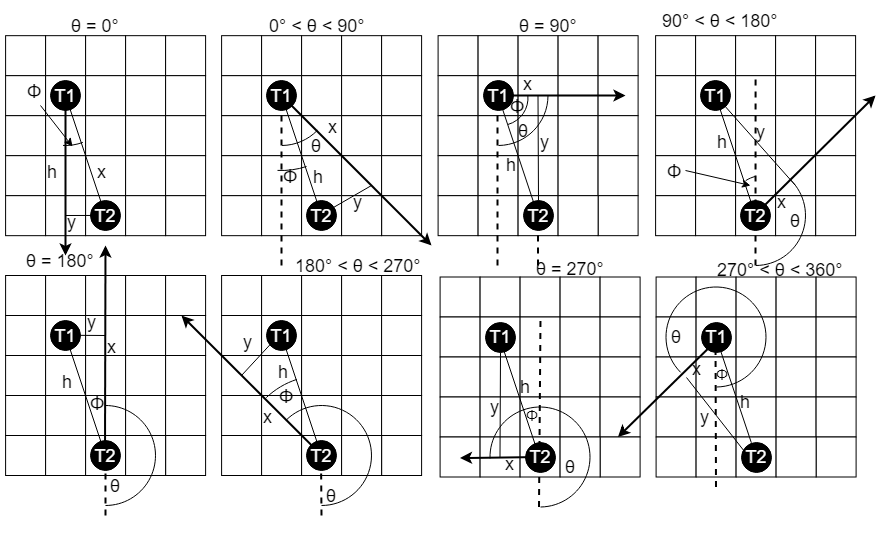
\includegraphics[width=\linewidth]{Figures/1142.png}
        \caption{Schematics of a worst configuration of a 1km by 1km wind farm with two wind turbines located at $(1,1)$ and $(4,2)$ for different wind directions.}
        \label{sampleSmall6}
    \end{figure}
    
    The manual computation of line segments $x$, $y$ from Figure \ref{sampleSmall4} and the resulting radius of the wake $r$ are shown below. If for the any wind direction where the resulting radius $r$ of the wake at a distance of $x$ is less than the length of $y$, then the wind speed of both wind turbines is both $u_1=u_2=12m/s$ and the power output of each is $P_1=P_2=518.400kW$.
    \begin{itemize}
\item $\theta=0^o$
	\begin{align*}%THETA=0
		x_{[\theta=0^o]} &=(632.456m) cos\left| (0^o\%90^o) - 18.435^o \right|  =600.0\;meters \\
		y_{[\theta=0^o]} &=(632.456m) sin\left| (0^o\%90^o) - 18.435^o \right|  =200.1\;meters \\
		r(600.0m) &=(0.32679491924311227)(600.0m)+20m  =216.77\;meters\\
		u_{2[\theta=0^o]} &=(12m/s)\left( 1-2(0.326795)\left( \frac{27.881}{27.881+(0.9437)(600.0m)} \right)^2 \right) =11.146\;m/s \\
		P_{2[\theta=0^o]} &=0.3(11.146m/s)^3  =415.411\;kiloWatts
\end{align*}
\item $\theta=10^o$
	\begin{align*}%THETA=10
		x_{[\theta=10^o]} &=(632.456m) cos\left| (10^o\%90^o) - 18.435^o \right|  =625.615\;meters \\
		y_{[\theta=10^o]} &=(632.456m) sin\left| (10^o\%90^o) - 18.435^o \right|  =92.773\;meters \\
		r(625.615m) &=(0.32679491924311227)(625.615m)+20m  =224.448\;meters\\
		u_{2[\theta=10^o]} &=(12m/s)\left( 1-2(0.326795)\left( \frac{27.881}{27.881+(0.9437)(625.615m)} \right)^2 \right) =11.193\;m/s \\
		P_{2[\theta=10^o]} &=0.3(11.193m/s)^3  =420.689\;kiloWatts
\end{align*}
\item $\theta=20^o$
	\begin{align*}%THETA=20
		x_{[\theta=20^o]} &=(632.456m) cos\left| (20^o\%90^o) - 18.435^o \right|  =632.22\;meters \\
		y_{[\theta=20^o]} &=(632.456m) sin\left| (20^o\%90^o) - 18.435^o \right|  =17.273\;meters \\
		r(632.22m) &=(0.32679491924311227)(632.22m)+20m  =226.606\;meters\\
		u_{2[\theta=20^o]} &=(12m/s)\left( 1-2(0.326795)\left( \frac{27.881}{27.881+(0.9437)(632.22m)} \right)^2 \right) =11.204\;m/s \\
		P_{2[\theta=20^o]} &=0.3(11.204m/s)^3  =421.93\;kiloWatts
\end{align*}
\item $\theta=30^o$
	\begin{align*}%THETA=30
		x_{[\theta=30^o]} &=(632.456m) cos\left| (30^o\%90^o) - 18.435^o \right|  =619.616\;meters \\
		y_{[\theta=30^o]} &=(632.456m) sin\left| (30^o\%90^o) - 18.435^o \right|  =126.794\;meters \\
		r(619.616m) &=(0.32679491924311227)(619.616m)+20m  =222.487\;meters\\
		u_{2[\theta=30^o]} &=(12m/s)\left( 1-2(0.326795)\left( \frac{27.881}{27.881+(0.9437)(619.616m)} \right)^2 \right) =11.182\;m/s \\
		P_{2[\theta=30^o]} &=0.3(11.182m/s)^3  =419.45\;kiloWatts
\end{align*}
\item $\theta=40^o$
	\begin{align*}%THETA=40
		x_{[\theta=40^o]} &=(632.456m) cos\left| (40^o\%90^o) - 18.435^o \right|  =588.185\;meters \\
		y_{[\theta=40^o]} &=(632.456m) sin\left| (40^o\%90^o) - 18.435^o \right|  =232.463\;meters \\
		r(588.185m) &=(0.32679491924311227)(588.185m)+20m  =212.216\;meters\end{align*}
\item $\theta=50^o$
	\begin{align*}%THETA=50
		x_{[\theta=50^o]} &=(632.456m) cos\left| (50^o\%90^o) - 18.435^o \right|  =538.882\;meters \\
		y_{[\theta=50^o]} &=(632.456m) sin\left| (50^o\%90^o) - 18.435^o \right|  =331.69\;meters \\
		r(538.882m) &=(0.32679491924311227)(538.882m)+20m  =196.104\;meters\end{align*}
\item $\theta=60^o$
	\begin{align*}%THETA=60
		x_{[\theta=60^o]} &=(632.456m) cos\left| (60^o\%90^o) - 18.435^o \right|  =473.206\;meters \\
		y_{[\theta=60^o]} &=(632.456m) sin\left| (60^o\%90^o) - 18.435^o \right|  =419.615\;meters \\
		r(473.206m) &=(0.32679491924311227)(473.206m)+20m  =174.641\;meters\end{align*}
\item $\theta=70^o$
	\begin{align*}%THETA=70
		x_{[\theta=70^o]} &=(632.456m) cos\left| (70^o\%90^o) - 18.435^o \right|  =393.151\;meters \\
		y_{[\theta=70^o]} &=(632.456m) sin\left| (70^o\%90^o) - 18.435^o \right|  =495.412\;meters \\
		r(393.151m) &=(0.32679491924311227)(393.151m)+20m  =148.48\;meters\end{align*}
\item $\theta=80^o$
	\begin{align*}%THETA=80
		x_{[\theta=80^o]} &=(632.456m) cos\left| (80^o\%90^o) - 18.435^o \right|  =301.151\;meters \\
		y_{[\theta=80^o]} &=(632.456m) sin\left| (80^o\%90^o) - 18.435^o \right|  =556.155\;meters \\
		r(301.151m) &=(0.32679491924311227)(301.151m)+20m  =118.415\;meters\end{align*}
\item $\theta=90^o$
	\begin{align*}%THETA=90
		x_{[\theta=90^o]} &=(632.456m) cos\left| 90^o - 18.435^o \right|  =200.1\;meters \\
		y_{[\theta=90^o]} &=(632.456m) sin\left| 90^o - 18.435^o \right|  =600.0\;meters \\
		r(200.1m) &=(0.32679491924311227)(200.1m)+20m  =85.392\;meters\end{align*}
\item $\theta=100^o$
	\begin{align*}%THETA=100
		x_{[\theta=100^o]} &=(632.456m) cos\left| (100^o\%90^o) - 18.435^o \right|  =625.615\;meters \\
		y_{[\theta=100^o]} &=(632.456m) sin\left| (100^o\%90^o) - 18.435^o \right|  =92.773\;meters \\
		r(625.615m) &=(0.32679491924311227)(625.615m)+20m  =224.448\;meters\end{align*}
\item $\theta=110^o$
	\begin{align*}%THETA=110
		x_{[\theta=110^o]} &=(632.456m) cos\left| (110^o\%90^o) - 18.435^o \right|  =632.22\;meters \\
		y_{[\theta=110^o]} &=(632.456m) sin\left| (110^o\%90^o) - 18.435^o \right|  =17.273\;meters \\
		r(632.22m) &=(0.32679491924311227)(632.22m)+20m  =226.606\;meters\end{align*}
\item $\theta=120^o$
	\begin{align*}%THETA=120
		x_{[\theta=120^o]} &=(632.456m) cos\left| (120^o\%90^o) - 18.435^o \right|  =619.616\;meters \\
		y_{[\theta=120^o]} &=(632.456m) sin\left| (120^o\%90^o) - 18.435^o \right|  =126.794\;meters \\
		r(619.616m) &=(0.32679491924311227)(619.616m)+20m  =222.487\;meters\end{align*}
\item $\theta=130^o$
	\begin{align*}%THETA=130
		x_{[\theta=130^o]} &=(632.456m) cos\left| (130^o\%90^o) - 18.435^o \right|  =588.185\;meters \\
		y_{[\theta=130^o]} &=(632.456m) sin\left| (130^o\%90^o) - 18.435^o \right|  =232.463\;meters \\
		r(588.185m) &=(0.32679491924311227)(588.185m)+20m  =212.216\;meters\end{align*}
\item $\theta=140^o$
	\begin{align*}%THETA=140
		x_{[\theta=140^o]} &=(632.456m) cos\left| (140^o\%90^o) - 18.435^o \right|  =538.882\;meters \\
		y_{[\theta=140^o]} &=(632.456m) sin\left| (140^o\%90^o) - 18.435^o \right|  =331.69\;meters \\
		r(538.882m) &=(0.32679491924311227)(538.882m)+20m  =196.104\;meters\end{align*}
\item $\theta=150^o$
	\begin{align*}%THETA=150
		x_{[\theta=150^o]} &=(632.456m) cos\left| (150^o\%90^o) - 18.435^o \right|  =473.206\;meters \\
		y_{[\theta=150^o]} &=(632.456m) sin\left| (150^o\%90^o) - 18.435^o \right|  =419.615\;meters \\
		r(473.206m) &=(0.32679491924311227)(473.206m)+20m  =174.641\;meters\end{align*}
\item $\theta=160^o$
	\begin{align*}%THETA=160
		x_{[\theta=160^o]} &=(632.456m) cos\left| (160^o\%90^o) - 18.435^o \right|  =393.151\;meters \\
		y_{[\theta=160^o]} &=(632.456m) sin\left| (160^o\%90^o) - 18.435^o \right|  =495.412\;meters \\
		r(393.151m) &=(0.32679491924311227)(393.151m)+20m  =148.48\;meters\end{align*}
\item $\theta=170^o$
	\begin{align*}%THETA=170
		x_{[\theta=170^o]} &=(632.456m) cos\left| (170^o\%90^o) - 18.435^o \right|  =301.151\;meters \\
		y_{[\theta=170^o]} &=(632.456m) sin\left| (170^o\%90^o) - 18.435^o \right|  =556.155\;meters \\
		r(301.151m) &=(0.32679491924311227)(301.151m)+20m  =118.415\;meters\end{align*}
    \end{itemize}
    
    For the rest of the wind directions ($180^o\leq \theta<360^o$), the power output of each wind wind turbines should interchange for opposite angles. For instance, the power output $P_{1[\theta=0^o]}$ and $P_{2[\theta=0^o]}$ of the wind turbines would be the same as the power output $P_{2[\theta=180^o]}$ and $P_{1[\theta=180^o]}$, respectively. That is,
    \begin{align*}
        P_{1[\theta=0^o]} = P_{2[\theta=180^o]} = 415.433\;kiloWatts \\
        P_{2[\theta=0^o]} = P_{1[\theta=180^o]} = 518.400\;kiloWatts
    \end{align*}
    
    The same computations were made using a computer and the computed values are shown in Table \ref{summaryAvg3}.
    
    %T1: (1,1) T2: (4,2)
    %h: 632.4551 phi: 0.0     P_tot=1014.8000494981015
    \singlespacing
    \begin{table}[H]
        \centering
        \begin{tabular}{|c|c|c|c|c|c|c|c|c|} \hline
    $\theta$ &$x$ &$y$ &$r$ &$u_1$ &$u_2$ &$P_1$ &$P_2$ &$P_1+P_2$ \\ \hline
$0^o$	&600.000	&200.000	&216.077	&12.000	&11.146	&518.400	&415.433	&933.833 \\ \hline
$10^o$	&625.614	&92.773	&224.448	&12.000	&11.193	&518.400	&420.691	&939.091 \\ \hline
$20^o$	&632.220	&17.274	&226.606	&12.000	&11.204	&518.400	&421.983	&940.383 \\ \hline
$30^o$	&619.615	&126.795	&222.487	&12.000	&11.182	&518.400	&419.495	&937.895 \\ \hline
$40^o$	&588.184	&232.464	&212.216	&12.000	&12.000	&518.400	&518.400	&1036.800 \\ \hline
$50^o$	&538.881	&331.069	&196.104	&12.000	&12.000	&518.400	&518.400	&1036.800 \\ \hline
$60^o$	&473.205	&419.615	&174.641	&12.000	&12.000	&518.400	&518.400	&1036.800 \\ \hline
$70^o$	&393.151	&495.412	&148.480	&12.000	&12.000	&518.400	&518.400	&1036.800 \\ \hline
$80^o$	&301.150	&556.155	&118.414	&12.000	&12.000	&518.400	&518.400	&1036.800 \\ \hline
$90^o$	&200.000	&600.000	&85.359	&12.000	&12.000	&518.400	&518.400	&1036.800 \\ \hline
$100^o$	&625.614	&92.773	&224.448	&12.000	&12.000	&518.400	&518.400	&1036.800 \\ \hline
$110^o$	&632.220	&17.274	&226.606	&12.000	&12.000	&518.400	&518.400	&1036.800 \\ \hline
$120^o$	&619.615	&126.795	&222.487	&12.000	&12.000	&518.400	&518.400	&1036.800 \\ \hline
$130^o$	&588.184	&232.464	&212.216	&12.000	&12.000	&518.400	&518.400	&1036.800 \\ \hline
$140^o$	&538.881	&331.069	&196.104	&12.000	&12.000	&518.400	&518.400	&1036.800 \\ \hline
$150^o$	&473.205	&419.615	&174.641	&12.000	&12.000	&518.400	&518.400	&1036.800 \\ \hline
$160^o$	&393.151	&495.412	&148.480	&12.000	&12.000	&518.400	&518.400	&1036.800 \\ \hline
$170^o$	&301.150	&556.155	&118.414	&12.000	&12.000	&518.400	&518.400	&1036.800 \\ \hline
$180^o$	&600.000	&200.000	&216.077	&11.146	&12.000	&415.433	&518.400	&933.833 \\ \hline
$190^o$	&625.614	&92.773	&224.448	&11.193	&12.000	&420.691	&518.400	&939.091 \\ \hline
$200^o$	&632.220	&17.274	&226.606	&11.204	&12.000	&421.983	&518.400	&940.383 \\ \hline
$210^o$	&619.615	&126.795	&222.487	&11.182	&12.000	&419.495	&518.400	&937.895 \\ \hline
$220^o$	&588.184	&232.464	&212.216	&12.000	&12.000	&518.400	&518.400	&1036.800 \\ \hline
$230^o$	&538.881	&331.069	&196.104	&12.000	&12.000	&518.400	&518.400	&1036.800 \\ \hline
$240^o$	&473.205	&419.615	&174.641	&12.000	&12.000	&518.400	&518.400	&1036.800 \\ \hline
$250^o$	&393.151	&495.412	&148.480	&12.000	&12.000	&518.400	&518.400	&1036.800 \\ \hline
$260^o$	&301.150	&556.155	&118.414	&12.000	&12.000	&518.400	&518.400	&1036.800 \\ \hline
$270^o$	&200.000	&600.000	&85.359	&12.000	&12.000	&518.400	&518.400	&1036.800 \\ \hline
$280^o$	&625.614	&92.773	&224.448	&12.000	&12.000	&518.400	&518.400	&1036.800 \\ \hline
$290^o$	&632.220	&17.274	&226.606	&12.000	&12.000	&518.400	&518.400	&1036.800 \\ \hline
$300^o$	&619.615	&126.795	&222.487	&12.000	&12.000	&518.400	&518.400	&1036.800 \\ \hline
$310^o$	&588.184	&232.464	&212.216	&12.000	&12.000	&518.400	&518.400	&1036.800 \\ \hline
$320^o$	&538.881	&331.069	&196.104	&12.000	&12.000	&518.400	&518.400	&1036.800 \\ \hline
$330^o$	&473.205	&419.615	&174.641	&12.000	&12.000	&518.400	&518.400	&1036.800 \\ \hline
$340^o$	&393.151	&495.412	&148.480	&12.000	&12.000	&518.400	&518.400	&1036.800 \\ \hline
$350^o$	&301.150	&556.155	&118.414	&12.000	&12.000	&518.400	&518.400	&1036.800 \\ \hline
        \end{tabular}
        \caption{Summary of the computation of $x$ (in meters), $y$ (in meters), the resulting radius of the wake $r$ (in meters), wind speed at each wind turbine $u_1$ $u_1$ (in m/s), the power output of each wind turbine $P_1$ $P_1$ (in kiloWatts) of two wind turbines located at $(1,1)$ and $(4,2)$ respectively on a 1km by 1km wind farm, and the total power output of the whole wind farm (in kiloWatts).}
        \label{summaryAvg3}
    \end{table}
    \doublespacing
    
    Since each wind direction's existence throughout the year is even, the fraction of occurrence of each wind direction is $\frac{1}{36}$. Therefore, the total annual power output of the whole wind farm with the current configuration would be
    \begin{align*}
        P_{tot}
        &= \sum_{\theta=0^o}^{350^o} \left( P_{1[\theta]} + P_{2[\theta]} \right) \cdot \frac{1}{36} \\
        &= \frac{1}{36}\left( P_{1[\theta=0^o]} + P_{2[\theta=0^o]} \right) + \frac{1}{36}\left( P_{1[\theta=10^o]} + P_{2[\theta=10^o]} \right) +...+ \frac{1}{36}\left( P_{1[\theta=350^o]} + P_{2[\theta=350^o]} \right) \\
        &= \frac{1}{36}\cdot\left( 518.4kW+415.433kW \right) + \frac{1}{36}\cdot\left( 518.4kW +420.691kW \right) +...+ \frac{1}{36}\cdot\left(  518.4kW + 518.4kW \right) \\
        &=1014.800\;kiloWatts
    \end{align*}
    
\subsection{Configurations of Three Wind Turbines}
    Since it is not always the case that there is only a single wake interaction, it is important to take multiple wake interactions into consideration. Note that multiple wake interactions happen for wind farms with at least three wind turbines installed. Consider the same small scale version of the problem but with three wind turbines namely $T_1$, $T_2$ and $T_3$. With these three wind turbines, the following scenarios can happen.
    \begin{enumerate}
        \item Wind turbines $T_1$, $T_2$ and $T_3$ does not affect each other.
        \item Wind turbines $T_2$ and $T_3$ are affected by the wake of wind turbine $T_1$.
        \item Wind turbine $T_3$ is affected by the wakes of wind turbines $T_1$ and $T_2$.
        \item Wind turbine $T_3$ is affected by the wake of wind turbine $T_2$ and wind turbine $T_2$ is affected by the wake of wind turbine $T_1$.
    \end{enumerate}
    where the second scenario exhibits single wake interaction while the third and fourth scenarios exhibit multiple wake interactions.
    
    To compute the wind speed experienced by wind turbines influenced by multiple wake interactions is to divide the multiple wake interaction into single ones, that is, determine the wind speed experienced by a wind turbine with respect to the wake effect of every upstream wind turbines. Consider the three wind turbines $T_1$, $T_2$ and $T_3$ where the upstream wind turbines $T_1$ and $T_2$ cause wake effect on the downstream wind turbine $T_3$. Let $u_\infty$ be the undisturbed wind inflow, $u_1$, $u_2$ and $u_3$ are wind speeds experienced by the wind turbines $T_1$, $T_2$ and $T_3$ respectively. Even if $T_1$ and $T_2$ are both upstream wind turbines, it does not mean that these two wind turbines experience the undisturbed wind speed. Using the Sum of Squares method, the computation of the wind speed $u_3$ of the the downstream wind turbine $T_3$ is shown below.
    \begin{align*}
        \left( 1-\frac{u_i}{u_\infty} \right)^2 &=\sum_{j=1}^{n} \left( 1-\frac{u_{ij}}{u_j} \right)^2 \\
        \left( 1-\frac{u_i}{u_\infty} \right) &= \sqrt{\sum_{j=1}^{n} \left( 1-\frac{u_{ij}}{u_j} \right)^2} \\
        u_i &= u_\infty\left( 1-\sqrt{\sum_{j=1}^{n} \left( 1-\frac{u_{ij}}{u_j} \right)^2} \right) \\
        u_3 &= u_\infty\left( 1-\sqrt{\left( 1-\frac{u_{31}}{u_1} \right)^2 + \left( 1-\frac{u_{32}}{u_2} \right)^2} \right)
    \end{align*}
    where $u_{31}$ is the expected wind speed at wind turbine $T_3$ due to the wake of wind turbine $T_1$ and $u_{32}$ is the expected wind speed at wind turbine $T_3$ due to the wake of wind turbine $T_2$. $u_{31}$ and $u_{32}$ can be computed as
    \begin{align*}
        u_{31} = u_\infty \left[ 1-2a\left( \frac{r_1}{r_1+\beta x_{31}} \right)^2 \right] \\
        u_{32} = u_\infty \left[ 1-2a\left( \frac{r_1}{r_1+\beta x_{32}} \right)^2 \right]
    \end{align*}
    where $x_{31}$ is the distance between $T_3$ and $T_1$ with respect to the direction of the wind and $x_{32}$ is the distance between $T_3$ and $T_2$ with respect to the direction of the wind.
    
    For the first scenario mentioned, the sum of square method should still work considering that the wind speed experienced by three wind turbines is the undisturbed wind inflow. To prove, let $u_1=u_2=u_\infty$ and it is needed to show that $u_3=u_\infty$. Since wind turbines $T_1$ and $T_2$ have no wake interaction, and the wind turbines $T_1$ and $T_3$ also have no wake interaction, then
    \begin{align*}
        u_{31}=u_{32}=u_\infty
    \end{align*}
    Then, it follows that
    \begin{align*}
        u_3 &= u_\infty\left( 1-\sqrt{\left( 1-\frac{u_{31}}{u_1} \right)^2 + \left( 1-\frac{u_{32}}{u_2} \right)^2} \right) \\
        u_3 &= u_\infty\left( 1-\sqrt{\left( 1-\frac{u_\infty}{u_\infty} \right)^2 + \left( 1-\frac{u_\infty}{u_\infty} \right)^2} \right) \\
        u_3 &= u_\infty\left( 1-\sqrt{\left( 1-1 \right)^2 + \left( 1-1 \right)^2} \right) \\
        u_3 &= u_\infty\left( 1-\sqrt{0 + 0} \right) \\
        u_3 &= u_\infty\left( 1 \right) \\
        u_3 &= u_\infty
    \end{align*} \hfill $\blacksquare$
    
    For example, let there be three wind turbines $T_1$, $T_2$ and $T_3$ installed on the same 1km by 1km wind farm with coordinates $(0,0)$, $(2,2)$ and $(3,4)$ respectively, a wind direction of $0^o$ and a wind speed of $12m/s$. First is to find the three pairs to determine if there are any single wake interactions. The pairs for this example would be $\{T_1,T_2\}$, $\{T_1,T_3\}$ and $\{T_2,T_3\}$. For each pair of wind turbines, the computation of  y-values ($y_{12}$, $y_{13}$, $y_{23}$), and the resulting radius of the individual wakes ($r_{12}$, $r_{13}$, $r_{23}$) are shown below.
    \begin{align*}
        y_{12}
        &=200m\cdot \left( \sqrt{(0-2)^2+(0-2)^2} \right)sin \left| (0^o\;mod\;90^o) - tan^{-1}\left|\frac{0-2}{0-2}\right| \right| \\
        &=\left( 565.685m \right)(0.707^o) \\
        &= 400\;meters
    \end{align*}
    \begin{align*}
        y_{13}
        &=200m\cdot \left( \sqrt{(0-3)^2+(0-4)^2} \right)sin \left| (0^o\;mod\;90^o) - tan^{-1}\left|\frac{0-4}{0-3}\right| \right| \\
        &=\left( 1000.000m \right)(0.800^o) \\
        &= 800.000\;meters
    \end{align*}
    \begin{align*}
        y_{23}
        &=200m\cdot \left( \sqrt{(2-3)^2+(2-4)^2} \right)sin \left| (0^o\;mod\;90^o) - tan^{-1}\left|\frac{2-4}{2-3}\right| \right| \\
        &=\left( 447.214m \right)(0.894^o) \\
        &= 400.000\;meters
    \end{align*}
    \begin{align*}
        r_{12}
        &= ax+r_o \\
        &= (0.326794)\left( 200m\cdot \left( \sqrt{(0-2)^2+(0-2)^2} \right)cos \left| (0^o\;mod\;90^o) - tan^{-1}\left|\frac{0-4}{0-3}\right| \right| \right) + 20m \\
        &=(0.326794)(400.000m)+20m \\
        &= 150.718\;meters
    \end{align*}
    \begin{align*}
        r_{13}
        &= ax+r_o \\
        &= (0.326794)\left( 200m\cdot \left( \sqrt{(0-3)^2+(0-4)^2} \right)cos \left| (0^o\;mod\;90^o) - tan^{-1}\left|\frac{0-4}{0-3}\right| \right| \right) + 20m \\
        &=(0.326794)(800.000m)+20m \\
        &= 281.435\;meters
    \end{align*}
    \begin{align*}
        r_{23}
        &= ax+r_o \\
        &= (0.326794)\left( 200m\cdot \left( \sqrt{(2-3)^2+(2-4)^2} \right)cos \left| (0^o\;mod\;90^o) - tan^{-1}\left|\frac{0-4}{0-3}\right| \right| \right) + 20m \\
        &=(0.326794)(200.000m)+20m \\
        &= 85.359\;meters
    \end{align*}
    Since every y-values is not less than the respective resulting radius of each pair of wind turbines, it means that every wind turbine is not affected by the wake of any other wind turbines on the wind farm. Therefore, there are no wake interactions between the wind turbines $T_1$, $T_2$ and $T_3$. With that, given the wind speed of $12m/s$, the power output of each wind turbine is 518.400 kiloWatts, giving a total power output for $\theta=0^o$ wind direction of
	\begin{align*}
		P_{tot[\theta=0^o]} &= 518.400kW + 518.400kW + 518.400kW \\
		&=1555.200\;kiloWatts
	\end{align*}
    
    The second scenario mentioned would happen if the three wind turbine $T_1$, $T_2$, and $T_3$ are located at $(0,1)$, $(1,0)$ and $(4,4)$ respectively where the wind blows at $\theta=220^o$. For each pair of wind turbines, the computation of  y-values ($y_{12}$, $y_{13}$, $y_{23}$), and the resulting radius of the individual wakes ($r_{12}$, $r_{13}$, $r_{23}$) are shown below.
    \begin{align*}
        y_{12}
        &=200m\cdot \left( \sqrt{(0-1)^2+(1-0)^2} \right) sin \left| (220^o\;mod\;90^o) - tan^{-1}\left|\frac{1-0}{0-1}\right| \right| \\
        &=\left( 282.843m \right)(0.087^o) \\
        &= 24.607\;meters
    \end{align*}
    \begin{align*}
        y_{13}
        &=200m\cdot \left( \sqrt{(0-4)^2+(1-4)^2} \right) sin \left| (220^o\;mod\;90^o) - tan^{-1}\left|\frac{1-4}{0-4}\right| \right| \\
        &=\left( 1000.000m \right)(0.055^o) \\
        &= 54.602\;meters
    \end{align*}
    \begin{align*}
        y_{23}
        &=200m\cdot \left( \sqrt{(1-4)^2+(0-4)^2} \right) sin \left| (220^o\;mod\;90^o) - tan^{-1}\left|\frac{0-4}{1-4}\right| \right| \\
        &=\left( 1000.000m \right)(0.227^o) \\
        &= 227.161\;meters
    \end{align*}
    \begin{align*}
        r_{12}
        &= ax+r_o \\
        &= (0.326794)\left( 200m\cdot \left( \sqrt{(0-1)^2+(1-0)^2} \right)cos \left| (220^o\;mod\;90^o) - tan^{-1}\left|\frac{1-0}{0-1}\right| \right|  \right) + 20m \\
        &=(0.326794)(281.766m)+20m \\
        &= 112.080\;meters
    \end{align*}
    \begin{align*}
        r_{13}
        &= ax+r_o \\
        &= (0.326794)\left( 200m\cdot \left( \sqrt((0-4)^2+{1-4)^2} \right)cos \left| (220^o\;mod\;90^o) - tan^{-1}\left|\frac{1-4}{0-4}\right| \right| \right) + 20m \\
        &=(0.326794)(998.508m)+20m \\
        &= 346.307\;meters
    \end{align*}
    \begin{align*}
        r_{23}
        &= ax+r_o \\
        &= (0.326794)\left( 200m\cdot \left( \sqrt{(1-4)^2+(0-4)^2} \right)cos \left| (220^o\;mod\;90^o) - tan^{-1}\left|\frac{0-4}{1-4}\right| \right| \right) + 20m \\
        &=(0.326794)(973.857m)+20m \\
        &= 338.251\;meters
    \end{align*}
    
It is shown that the y-values of the wind turbine pairs are less than than the r-values. However, this doesn't mean that all pairs have wake interactions. Note that the formulas for x-value and, y-value only work if one turbine is covered by the swept area of the other wind turbine. From the the current configuration of wind turbines $T-1$, $T_2$ and $T_3$, the pair $\{T_1,T_2\}$ cannot show wake interaction as neither of them is covered by the swept area of the other. Hence, only the pairs $\{T_1,T_3\}$ and $\{T_2,T_3\}$ have single wake interactions where the wind turbine $T_3$ is the upstream wind turbine. With/that, the wind speed at wind turbine $T_3$ is $12\;m/s$ while the wind speeds at $T_1$ and $T_2$ are
	\begin{align*}
        u_{1} &= u_\infty \left[ 1-2(0.326794)\left( \frac{27.881m}{27.881m+(0.0943696) (998.508m)} \right)^2 \right] \\
        &=11.591\;m/s
    \end{align*}
    \begin{align*}
        u_{2} &= u_\infty \left[ 1-2(0.326794)\left( \frac{27.881m}{27.881m+(0.0943696) (973.857m)} \right)^2 \right] \\
        &=11.575\;m/s
    \end{align*}
with wind power output of
	\begin{align*}
		P_1=0.3(11.591m/s)^3 \\
		=467.180\;kiloWatts
	\end{align*}
	\begin{align*}
		P_2=0.3(11.575m/s)^3 \\
		=465.248\;kiloWatts
	\end{align*}
giving a total power output for $\theta=220^o$ wind direction of
	\begin{align*}
		P_{tot[\theta=220^o]} &= 467.180kW + 465.248kW + 518.400kW \\
		&=1450.828\;kiloWatts
	\end{align*}
    
    Changing the wind direction to $\theta=40^o$ would portray the third scenario. The y-values and r-values for each pair of wind turbines would be the same since the new wind direction is the opposite of the previous one, that is, the wind is reversed. Thus, the single wake interactions would exist for wind turbines pairs $\{T_1,T_3\}$ and $\{T_2,T_3\}$ where the wind turbine $T_3$ is the downstream wind turbine for both pairs. The expected wind speed at $T_3$ due to the wake of individual wakes of win turbines $T_1$ and $T_2$ are as follow.
    \begin{align*}
        u_{31} &= u_\infty \left[ 1-2(0.326794)\left( \frac{27.881m}{27.881m+(0.0943696) (998.508m)} \right)^2 \right] \\
        &=11.591\;m/s
    \end{align*}
    \begin{align*}
        u_{32} &= u_\infty \left[ 1-2(0.326794)\left( \frac{27.881m}{27.881m+(0.0943696) (973.857m)} \right)^2 \right] \\
        &=11.575\;m/s
    \end{align*}
    Then, the wind speed at $T_3$ due to the wakes of wind turbines $T_1$ and $T_2$ is as follows.
    \begin{align*}
        u_3 &= u_\infty\left( 1-\sqrt{\left( 1-\frac{u_{31}}{u_1} \right)^2 + \left( 1-\frac{u_{32}}{u_2} \right)^2} \right) \\
        &= (12m/s)\left( 1-\sqrt{\left( 1-\frac{11.591m/s}{12.000m/s} \right)^2 + \left( 1-\frac{11.575m/s}{12.000m/s} \right)^2} \right) \\
        &= 11.410\;m/s
    \end{align*}
    Hence, the power output of wind turbine $T_3$ at wind direction $\theta=40^o$ is
    \begin{align*}
        P_{3[\theta=40^o]} &= 0.3(11.410m/s)^3 \\
        P_{3[\theta=40^o]} &= 445.653\;kiloWatts
    \end{align*}
    while the upstream wind turbines $T_1$ and $T_2$ have power outputs of
    \begin{align*}
        P_{1[\theta=40^o]}=P_{2[\theta=40^o]} = 518.400\;kiloWatts
    \end{align*}
   giving a total power output for $\theta=40^o$ wind direction of
	\begin{align*}
		P_{tot[\theta=40^o]} &= 518.400kW + 518.400kW + 445.653kW \\
		&=1482.453\;kiloWatts
	\end{align*}
	
	Consider a configuration of three wind turbines where the wind turbines are align in row, say the locations for wind turbines $T_1$, $T_2$ and $T_3$ are at $(0,2)$, $(2,2)$ and $(4,2)$ where the wind blows at a direction of $\theta=0^o$. This would show the fourth scenario. From this, it is obvious the the x-values are 400 meters for wind turbine pairs $\{T_1,T_2\}$ and $\{T_2,T_3\}$, and 800 meters. Also, the y-value for every pair of wind turbines is always 0 meters because the three wind turbines aligned with the direction of the wind. With that, the wind speed and power output at wind turbine $T_1$ would be
	\begin{align*}
		u_{1[\theta=0^o]} &=12\;m/s \\
		P_{1[\theta=0^o]} &=518.400\;kiloWatts
	\end{align*}
while the wind turbine $T_2$ is affected by the wake of wind turbine $T_1$. Hence, the wind speed at $T_2$ would be
	\begin{align*}
        u_{2[\theta=0^o]} &= u_\infty \left[ 1-2(0.326794)\left( \frac{27.881m}{27.881m+(0.0943696) (400.000m)} \right)^2 \right] \\
        &=10.584\;m/s
    \end{align*}
where the power output of $T_2$ is
	\begin{align*}
        P_{2[\theta=0^o]} &= 0.3(10.584m/s)^3 \\
        P_{2[\theta=0^o]} &= 355.689\;kiloWatts
    \end{align*}
However, wind turbine $T_3$ is affected by the wake of both $T_1$ and $T_2$. The expected wind speeds at $T_3$ due to individual wakes of $T_1$ and $T_2$ are as follows.
	\begin{align*}
        u_{31} &= (12m/s) \left[ 1-2(0.326794)\left( \frac{27.881m}{27.881m+(0.0943696) (800.000m)} \right)^2 \right] \\
        &=11.429\;m/s
    \end{align*}
    \begin{align*}
        u_{32} &= (10.584m/s) \left[ 1-2(0.326794)\left( \frac{27.881m}{27.881m+(0.0943696) (400.000m)} \right)^2 \right] \\
        &=9.336\;m/s
    \end{align*}
Then, the wind speed at $T_3$ due to the wakes of wind turbines $T_1$ and $T_2$ is as follows.
    \begin{align*}
        u_3 &= u_\infty\left( 1-\sqrt{\left( 1-\frac{u_{31}}{u_1} \right)^2 + \left( 1-\frac{u_{32}}{u_2} \right)^2} \right) \\
        &= (12m/s)\left( 1-\sqrt{\left( 1-\frac{11.429m/s}{12.000m/s} \right)^2 + \left( 1-\frac{9.336m/s}{12.000m/s} \right)^2} \right) \\
        &= 9.275\;m/s
    \end{align*}
Hence, the power output of wind turbine $T_3$ at wind direction $\theta=0^o$ is
    \begin{align*}
        P_{3[\theta=0^o]} &= 0.3(9.275m/s)^3 \\
        &= 239.404\;kiloWatts
    \end{align*}
giving a total power output for $\theta=0^o$ wind direction of
	\begin{align*}
		P_{tot[\theta=0^o]} &= 518.400kW + 355.689kW + 239.404kW \\
		&=1113.493\;kiloWatts
	\end{align*}
	
	\subsubsection{Best Configuration}
	tetst